\documentclass{report}
\usepackage[extreme]{savetrees}
\usepackage{wrapfig}
\usepackage{chemformula}
\usepackage{graphicx}
\graphicspath{{./images/}}
\usepackage{amsthm}
\usepackage{siunitx}
\usepackage{url}
\usepackage{subfig}
\usepackage{lscape}
\usepackage{amsmath}
\usepackage{tikz}
\usepackage{mathdots}
\usepackage{epigraph}
\usepackage{yhmath}
\usepackage{cancel}
\usepackage{float}
\usepackage{color}
\usepackage{siunitx}
\usepackage{array}
\usepackage{multirow}
\usepackage{titlepic}
\usepackage{amssymb}
\usepackage{gensymb}
\usepackage{tabularx}
\usepackage{booktabs}
\usetikzlibrary{fadings}
\title{Marketing Training Report}
\author{Tuneer Bhattacherjee\\Employee Id: 514370\\BhattacherjeeT@indianoil.in}
\titlepic{
\includegraphics[width=5cm]{iocl_logo}}
\date{}
\makeindex
\begin{document}
	\maketitle
	\pagebreak
	\tableofcontents
	\pagebreak
	\listoffigures
	\pagebreak
	\listoftables
	\chapter{Sanand Bottling Plant}
	\section{Important Terms and Abbreviations}
	\begin{itemize}
		\item OISD= Oil Industry and Safety Directorate
		\item PESO= Petroleum and Explosives Safety Organization
		\item TT= Tanker Trucks
		\item Cavitation = Cavitation is a phenomenon in which rapid changes of pressure in a liquid lead to the formation of small vapor-filled cavities, in places where the pressure is relatively low.When subjected to higher pressure, these cavities, called "bubbles" or "voids", collapse and can generate an intense shock wave. These shock waves can damage pumps/motors.
		\item CFM= Cubic Feet per Minute
		\item SO= State Office
		\item HO= Head Office
		\item DOA= Delegation of Authority
		\item BCW= Blue Collar Workers
		\item VCB= Vacuum Circuit Breaker
		\item ACB= Air Circuit Breaker
		\item EB= Electricity Board
		\item T/F= Transformer
		\item CT= Current Transformer
		\item PT= Potential Transformer
		\item CB= Circuit Breaker
		\item SFU= Switch Fuse Unit (See Fig \ref{sfu})
		\item EP= Earthing Pit
		\item TLV= Threshold Limit Value
		\item LEL= Lower Explosive Limit
		\item UEL= Upper Explosive Limit
		\item BA= Breathing Apparatus
		\item STEL= Short Term Exposure Level
		\item TLD= Tank Lorry Decantation
		\item SRD= Stay Ring Defect
		\item FRD= Foot Ring Defect
	\end{itemize}
	\section{Sanand Bottling Plant - Day 1 (13.08.2019)}
	
	\subsection{Introduction to Sanand LPG Bottling Plant - Salient Points}
	\textit{Faculty: Shri. Joydev Ojha, DGM(P), Sanand BP}
	\begin{itemize}
		\item Due to low land prices and government push, this particular bottling plant has much more space than what is required under the OISD guidelines.
		\item In addition to that, there is a 66 acre buffer area which is not required anymore according to the latest OISD guidelines so, the plant "occupier" or location in charge Shri. Joydev Ojha, DGM(P) has decided to utilize it to benefit the corporation in the following ways:-
		\begin{itemize}
			\item A 8MW solar plant was established in the buffer area which generates about Rs.3 lacs of electricity per day, part of which is used up by the factory and part is distributed to other IOCL facilities via the grid. It is important to note that according to the some regulations in the Gujrat solar power consumption policy, IOCL at max can only generate 50\% of their net electricity demand if they wish to stay on grid and share their power with other IOCL facilities using the same. This facility covers 66 acre of the buffer area. 
			
			\item  A 2 acre lube storage facility (CFA). It is important to note here that lube being a high flashpoint product is an ``excluded product''. Therefore, storing it in buffer areas donot raise any safety concerns.
			
			\item 4 acres are being delegated to the pipelines division to facilitate the Kandla-Gorakhpur pipeline.
			
			
		\end{itemize}
		\item Product is sourced into the bottling plant using approximately 100 LPG TTs of 18-20 MTs from the following sources -
		\begin{itemize}
			\item Kandla port
			\item Pipawa port
			\item Varoda refinery
			\item Reliance refinery, Jamanagar
			\item Essar refinery, Jamnagar etc.
		\end{itemize}
	
		\item There are 8 TLDs which takes about 3-4 hours to completely decant all the trucks and this happens in about 4 batches a day.
		
		\item Storage of LPG is done as follows:-
		\begin{itemize}
			\item 3 Horton Spheres 1400 MT,1200 X 2 MT
			\item 1 Stationary Vessel ie. Bullet 150 X 4 MT
		\end{itemize}
		Therefore, net storage capacity = $1400+12 X 1200+150X4 = 4400 MT$
		\item Decantation is done via pressure difference using a vapour compressor in the following steps:-
		\begin{itemize}
			\item First vapour of TT is pressurized by taking vapour from vessel. This forces liquid LPG to move from TT to vessel.
			\item Then, liquid valve is closed and then vapour is sucked from the tanker using vapour suction.
		\end{itemize}
		This method is preferred over simply using pumps to pump the LPG from TT to vessel because if the pump pulls vapor by mistake, that will lead to cavitation.
		\item There are 3 carousels - 1400 cylinders/hour X 2 and 1600 cylinders per hour.
		\item The 3 carousels are fed by 3 pumps - 110 , 90, 36 X 2 CFM each with a max capacity of 6000 cylinders per month therefore, the net capacity would be approximately 18000 per month, but generally only about 15000 are required to be produced as per guidance from SO.
		\item The following requirement from SO side is generated by a computer model which takes the following factors into account -
		\begin{itemize}
			\item Bulk receiving cost
			\item Capacity of plant
			\item Demand from market
			\item Transportation cost from plant to market
		\end{itemize}
		\item There are 2 types of valves in cylinders ie. Self Closing Valve (SC) \ref{sc_valve}and Liquid Off Take Valves (LOT) \ref{lot_valve}.
		\item Delivery within 24 hours to distributor.
		\item There are baffle plates in LPG TTs to arrest momentum of the fluid thereby causing less hindrance to the driver.
	\end{itemize}
	\subsection{Roles and Responsibilities - Salient Points}
	\textit{Faculty: Shri. Joydev Ojha, DGM(P), Sanand BP}
	\begin{itemize}
		\item Occupier has he role responsibility and has the power of attorney
		\item The occupier then delegates the responsibility /authority to other officers below him via DOA guidelines.
		\item Finally the grass root users of official authority are Grade 'A' Officers who get the work done by the BCW in company payroll and contractors.
	\end{itemize}
	\subsection{LPG Plant Layout - Salient Points}
	\textit{Faculty: Shri. B.H. Bharti, SM(P), Sanand BP}
	\begin{itemize}
		\item There are four sizes of BPs based on net production per annum-
		\begin{enumerate}
			\item less than 6000 ---- Micro
			\item between 6000 to 22000 ---- Mini
			\item between 22000 to 68000 ---- Major
			\item greater than 68000 ---- Mega
		\end{enumerate}
		Based on information given above the average production per month of Sanand BP is 15000 therefore appx. production per annum 15000 X 12 = 180000 which is greater than 68000. Therefore, Sanand BP is a Mega Plant.2
		\item Vapour seals are used in water drains so that LPG vapour (which is heavier than air) cannot travel outside the plant licensed area where it can catch spark and ignite thereby causing grave fatalities and carry the ignition to plant and cause an even bigger calamity.
		\item Types of storage at any LPG facility can be as follows:-
		\begin{itemize}
			\item Above ground storage- Bullets, Horton Spheres, Mounded Storage
			\item Under ground storage
			\item Cavern storage
			\item Refrigerated storage tank @ \ang{-42}C and atm pressure
		\end{itemize}
		\item Minimum of 3 vessels are to be kept at a plant.
		\item Storage vessel should be filled upto 84-85\% to keep room for LPG expansion with change of temperature, failing this, risk of explosions due to expansions are considerably increased which renders such operating procedure ineffective and useless. 
		\item Mimimum compressor air pressure for carousel is 5.5 kg/cc and for the latest fully automatic carousel it is 6 kg/cc
		\item The following are the various types of LPG cylinders in the portfolio of IndianOil-Indane - (all are weight of LPG only)
		\begin{itemize}
			\item 5 kg (domestic/commercial)
			\item 14.2 kg (subsidized/non-subsidized domestic)
			\item 19 kg (commercial for hotels etc./nanocut for fabrication etc.)
			\item 47.5 kg (commercial for furnace, biscuit burners etc with SC or LOT valves/ domestic)
			\item 425 kg (only commercial)
		\end{itemize}
	\item The color coding for Indane cylinders is red for domestic and blue for commercial.
	\item Nanocut cylinders contain LPG along with an additive which gives rise to a sharp flame, which helps in cutting metal easily and accurately.
	\item The following are the truck capacities of the LPG cylinder trucks -306, 450, 504, 540 cylinders.
	\item SAP code for induction of new trucks - O4V1
	\item The bulk tankers incoming have the following capacities - 18 MT and 21 MT
	\item The following are defects for which cylinders are returned to IOCL from market and the corporation has to suitably compensate the distributor via credit according to policy \textbf{(Market Return Policy)}-
	\begin{itemize}
		\item Oversize/undersize valve
		\item Bung leak
		\item Underweight/overweight
		\item Broken pin
		\item Pin stuck up
		\item Water filled cylinder
		\item Body leak
		\item Other OMC (Oil Marketing Company) Cylinder
		\item Burnt cylinder
		\item SRD (Stay Ring Defect) / FRD (Foot Ring Defect)
	\end{itemize}
	\end{itemize}

	
	\section{Sanand Bottling Plant - Day 2 (14.08.2019)}
	\subsection{Electrical Systems - Salient Points}
	\textit{Faculty: Shri. Prakash Chand Meena, OO(P), Sanand BP}\\

	With respect to Fig \ref{bp_singlelinediag}, the following points should be noted:-
	\begin{itemize}
		\item VCB1 monitors the following - voltage, power factor, frequency, current and has ratings as defined in Table \ref{vcb1_nameplate}
		\item The VCB has the following components for operation - CTs, PTs and CBs.
		\item Inside any panel, the electrical power goes through the following equipment-s in order:- SFU (415 V), Fuse, Contactor(125 A rating), Thermal Relay (only for over current). See Fig \ref{sfu}.
		\item There are total 17 racks each with 2 sides and 6 units (as rows) on each side. So all in all there is accommodation for 17 X 2 X 6 = 228 equipment such as conveyer motor etc.
		\item All the control signals for the VCB and ACBs need 110 V DC supply as does the emergency lights. This is supplied by a DC distribution system as shown in Fig. \ref{dc_distribution}.
	\end{itemize}
	\begin{itemize}
		\item In the panels the following protection measures are present \textbf{Switch} to \textbf{Fuse}(Now replaced by \textbf{SFU} - Switch Fuse Unit See Fig \ref{sfu}) to \textbf{Contactor} to \textbf{Thermal Relay} to \textbf{Equipment}. The practical example of this can be seen in Fig \ref{inside_panel}.
		\item In tranformers, as we can see from Table \ref{sanand_isolation_tf_datacard}, \ref{sanand_stepdown_tf_datacard} there is a guaranteed rise of temperature of winding and oil upto \ang{55}C, therefore the high temperature alarm goes off at \ang{60}C and trips the transformers at \ang{90}C for oil OR winding overheating.
		\item Other that this, there is no inline protection for transformers such as differential protection (protection by Mertz-Price Circulating Current principle).
		\item However, for protection of transformers from Incipient faults, there are Buccholz Relays attached to each transformer. 
		\item For reactive power compensation there are capacitor banks which are switched on and off via thyristors with the help of a automatic VAR compensator which keeps the power factor above 0.96 by switching on as many capacitors as required. The following are the capacities of the compensators available (Total Capacity= 340 kVAR):-
		\begin{itemize}
			\item 25 kVAR X 13 = 325 kVAR
			\item 10 kVAR X 1  = 010 kVAR
			\item 5 kVAR X 1 =   005 kVAR
		\end{itemize}
		\item There are 3 types of earthing present in a bottling plant (or any industrial facility for that matter) - Neutral Earthing (for DG and TF), Lightning Earthing (for Buildings and other structures), Body Earthing (for every electrical equipment in the plant and 2 point earthing if operating voltage is more than 250 Volts). The earthing schemes as per OISD regulations are roughly described in Fig \ref{bp_earthing}
	\end{itemize}
	
	
	\subsection{LPG Plant Safety - Salient Points}
	\textit{Faculty: Shri. Umesh Malviya, OO(LPG-Safety), Sanand BP}\\
	\begin{itemize}
		\item Safety is the freedom from injury, death and damage.
		\item All accidents are preventable.
		\item Incident = Something wrong happened but no one was harmed or no damage was done whatsover.
		\item Near Miss = Some minor injury occurred or injury was just avoided.
		\item Accident = Someone died and some major property damage has occurred.
		\item Reasons for accidents are 88\% human error, 10\% unsafe condition and 2\% a combination of both.
		\item The fire triangle consists of 3 things required for a fire - product, air (oxygen) and spark. Therefore, just by removing any one of the three, fire can be stopped. However, that is not always the case for compounds like \textbf{Ethylene Oxide} which itself consists of oxygen, therefore the only was to stop the fire is to cut the fuel out of the equation.
		\item TLV for any chemical is a measure of how toxic it is to human beings. If the chemical concentration is more than the TLV then the max amount of time for which a person can operate in that environment without incurring serious damage is 8 hours. The TLV for LPG is 1000 ppm.
		\item All equipments present inside the licensed area have to be PESO approved.
		\item If the mixture of fuel and air is below LEL (1.9\% for LPG) then it will not burn due to lack of fuel and is considered ``too lean to burn", and if the mixture is above UEL then it will not burn due to lack of oxygen and is considered ``too rich to burn". Therefore, the danger lies when the concentration is between LEL and UEL.
		\item Using a fire extinguisher (PASS) - \textbf{P}ull the pin, \textbf{A}im at the base of fire, \textbf{S}queeze the trigger and \textbf{S}weep.
		\item There are 2 types of fire protection - Active and Passive Fire protection. Active fire protection is a group of systems that require some amount of action in order to work efficiently in the event of a fire eg. fire extinguishers, automatic sprinkler systems, alarms etc. Passive fire protection is a group of systems that compartmentalize a building through the use of fire-resistance rated walls and floors, keeping the fire from spreading quickly and providing time to escape for people in the building eg. fire doors,  photoluminescent egress path markers etc.
		\item There are 3 types of safety audits - Internal Safety Audit (Every 1 year), External audit by OISD (Every 5 years) and Suprise Audits.
		\item The expansion ratio of LPG is 1:250.
		\item The hazchem code for LPG is 2WE. See Fig \ref{hazchem} to know how to read hazchem signs. 2WE means that in case of an incident, fog of water must be sprayed, full protective clothing must be worn with Breathing Apparatus (BA), spill must be contained.
		\item Self Contained BA shows contained air pressure in bar. To convert it into minutes remaining, the shortcut formula is to remove the ending 0 and then add it to half of itself. For eg 300 bar means 30+15=45 mins, similarly 200 bar means 20+10=30mins.
		\item 
	\end{itemize}
	
	\section{Sanand Bottling Plant - Day 3 (16.08.2019)}
	
	\subsection{Supply \& Distribution - Salient Points}
	\textit{Faculty: Shri. Himanshu Jatav, OO(P), Sanand BP}\\
	\begin{itemize}
		\item Truck carrying cylinders have the following capacities :- 306/450/504 (no partial loads are given to any distributor)
		\item Under the current Market Return Policy in the MDG, the following forms grounds for return of cylinder from market:-
		\begin{itemize}
			\item Oversize or undersize valve
			\item Bung leak
			\item Underweight or overweight
			\item Broken pin
			\item Pin stuck up
			\item Water filled cylinder
			\item Body leak
			\item Other OMC cylinder 
			\item Burnt cylinder
			\item SRD or FRD
		\end{itemize}
	\end{itemize}
	
	\subsection{Bulk - Salient Points}
	\textit{Faculty: Shri. Shirish Rao, SM(P), Sanand BP}\\
	\begin{itemize}
		\item Bulk domestic product= 89000 MT
		\item Bulk international product= 94000 MT
		\item Supply for domestic from Kandla 
		\item Supply for only non domestic from Dumar
		\item Supply for domestic from Essar Oil Limited (EOL), Jamnagar and Reliance, Jamnagar
		\item +-200g allowed in Gross Weight-Tear Weight
		\item TLD tests performed - Visual inspection, Pneumatic Test, Hydrostatic Test, Electrical Continuity.
	\end{itemize}
	
	\section{Sanand Bottling Plant - Day 4 (17.08.2019)}
	\subsection{Stores - Salient Points}
	\textit{Faculty: Shri. Nitin Parwani, AM(P), Sanand BP}\\
	Store contains the following:-
	\begin{itemize}
		\item Project - Contains project materials when such projects are being performed - Compressor, DG, Lights etc.
		\item LPG Consumables - SC valve, Pressure Regulator, O-Ring, TES, Soap Solution, Safety Caps
		\item HSD - for DG sets
		\item Lube - lube oil, I5W40
		\item Revenue Maintenance - Conveyer material, bearing, solenoid valve.
	\end{itemize}
	
	\subsection{Shed Visit}
	The filling shed operation can be summarised by the following points:-
	\begin{itemize}
		\item Washing unit
		\item Drying unit
		\item Pre-O Ring Machine
		\item Carousel
		\item Check scale
		\item Weight correction unit
		\item Valve leak detector
		\item Post-O Ring Machine
		\item Water Bath
		\item Sealing Machine
		\item Purging Machine - Taking pressure to -0.365 kg/cm2, in order to aide filling of LPG.
	\end{itemize}
	The correct order of things can be seen in Fig \ref{lpg_flow}.
	\subsection{Closing Session - Salient Points}
	\textit{Faculty: Shri. Joydev Ojha, DGM(P), Sanand BP}\\
	\begin{itemize}
	\item CVT= Continuous Valve Testing which checks for both valve leak and o ring leak.
	\item CVT verifier is to check if CVT is working or not
	\item When a cylinder is beyond repair, the following steps are taken to discard it - 
	\begin{enumerate}
		\item Evacuation
		\item Depressurize
		\item Valve removal
		\item Degassing
		\item Sent for scraping
	\end{enumerate}
	\end{itemize}
	
	\clearpage
	\pagebreak
	\section{Tables}
	\begin{table}[h]
		\centering
		\begin{tabular}{@{}lll@{}}
			\toprule
			\textbf{S. No.} & \textbf{SPECIFICATION}   & \textbf{VALUE}    \\ \midrule
			1               & TYPE                     & VK 10J20          \\
			2               & SERIAL NUMBER            & 2639              \\
			3               & YEAR                     & 1995              \\
			4               & STANDARD                 & IS:13118 / IEC-56 \\
			5               & RATED FREQUENCY          & 50 Hz             \\
			6               & RATED VOLTAGE            & 12 kV             \\
			7               & RATED CURRENT            & 630               \\
			8               & Ins.LEVEL Imp.           & 75 kVp;P.F.28 kV  \\
			9               & RATED BREAKING CURRENT   & 20 kA             \\
			10              & RATED MAKING CURRENT     & 50 A (Peak)       \\
			11              & SUPPLY VOLTAGE CLOSING   & 110 V DC          \\
			12              & SUPPLY VOLTAGE TRIPPING  & 110 V DC          \\
			13              & RATED SHORT TIME CURRENT & 20 kA ( 3 secs)   \\
			14              & WEIGHT OF BREAKER        & 70 kg             \\ \bottomrule
		\end{tabular}
		\caption{VCB1 technical specifications made in technical collaboration with Toshiba Japan}
		\label{vcb1_nameplate}
	\end{table}
	\begin{table}[h]
		\centering
		\begin{tabular}{@{}lll@{}}
			\toprule
			\textbf{S. No.} & \textbf{Specification}       & \textbf{Value}             \\ \midrule
			1               & Specification                & IS 2028                    \\
			2               & Phase                        & 3                          \\
			3               & Frequency                    & 50Hz                       \\
			4               & Ambient Temperature          & 45 Degree C                \\
			5               & Max Temperature Allowed      & 55 Degree C                \\
			6               & Primary Winding              & 433 Volts +2.5\%+5\% DELTA \\
			7               & Secondary Winding            & 433 Volts STAR             \\
			8               & Primary Vpeak or Amplitude   & 266.67 Volts               \\
			9               & Secondary Vpeak or Amplitude & 266.67 Volts               \\
			10              & Impedance Volts              & 4.62\%                     \\
			11              & Oil                          & 330 l                      \\
			12              & Vector Group Ref.            & Dyn11                      \\
			13              & Cooling                      & ON/AN                      \\
			14              & KVol                         & 200                        \\
			15              & Insulation Class             & A                          \\
			16              & Type                         & DW                         \\
			17              & Weight                       & 1110 kg                    \\
			18              & Serial Number                & ABY-1-9                    \\ \bottomrule
		\end{tabular}
		\caption{Data card for the Isolation Transformer for the lighting equipment as mentioned in Fig \ref{bp_singlelinediag}}
		\label{sanand_isolation_tf_datacard}
	\end{table}
	\begin{table}[h]
		\centering
		\begin{tabular}{@{}lll@{}}
			\toprule
			\textbf{S. No.} & \textbf{Specifications}                                                 & \textbf{Value}                                      \\ \midrule
			1               & Standard                                                                & IS 2026-1977                                        \\
			2               & kVA Rating                                                              & \begin{tabular}[c]{@{}l@{}}1000\\  kVA\end{tabular} \\
			3               & HV Voltage Rating (No Load)                                             & 11000 Volts                                         \\
			4               & LV Voltage Rating (No Load)                                             & 433 Volts                                           \\
			5               & HV Current Rating                                                       & 52.5 A                                              \\
			6               & LV Current Rating                                                       & 1333 A                                              \\
			7               & No. of phases at HV and LV                                              & 3                                                   \\
			8               & Type of Cooling                                                         & ONAN                                                \\
			9               & Impedance Volts                                                         & 4.13\%                                              \\
			10              & Vector Group Reference                                                  & Dyn 11                                              \\
			11              & Core and Windings Weight                                                & 1520 kg                                             \\
			12              & Oil Weight                                                              & 740 kg                                              \\
			13              & Total Weight                                                            & 3260 kg                                             \\
			14              & Oil Quantity                                                            & 770 litres                                          \\
			15              & Year of Manufacture                                                     & 1995                                                \\
			16              & \begin{tabular}[c]{@{}l@{}}Max Temp Rise of Oil\\  and Wdg\end{tabular} & 55 degrees C                                        \\
			17              & Insulation Level                                                        & LI 75 AC 28/LI AC-3                                 \\ \bottomrule
		\end{tabular}
		\caption{Datacard for the main step down transformer connected to the Electricity Board in Fig \ref{bp_singlelinediag}}
		\label{sanand_stepdown_tf_datacard}
	\end{table}
	
	\clearpage
	\pagebreak
	\section{Figures}
	\begin{figure}[h]
		\centering
		\subfloat[][LOT Valve]{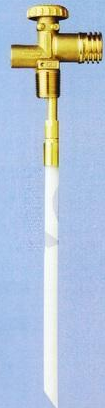
\includegraphics[height=5cm,width=5cm]{lot_valve}\label{lot_valve}}
		\subfloat[][SC Valve]{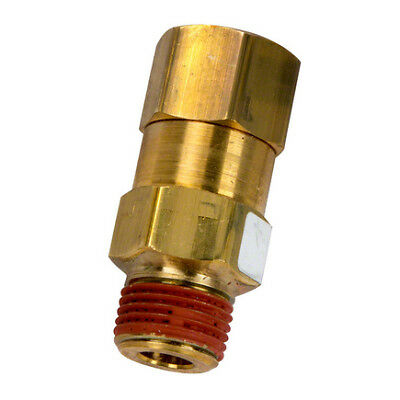
\includegraphics[height=5cm,width=5cm]{sc_valve}\label{sc_valve}}
		\caption{Types of valves attached to LPG cylinders}
		\label{lpg_valves}
	\end{figure}
	\begin{figure}[h]
		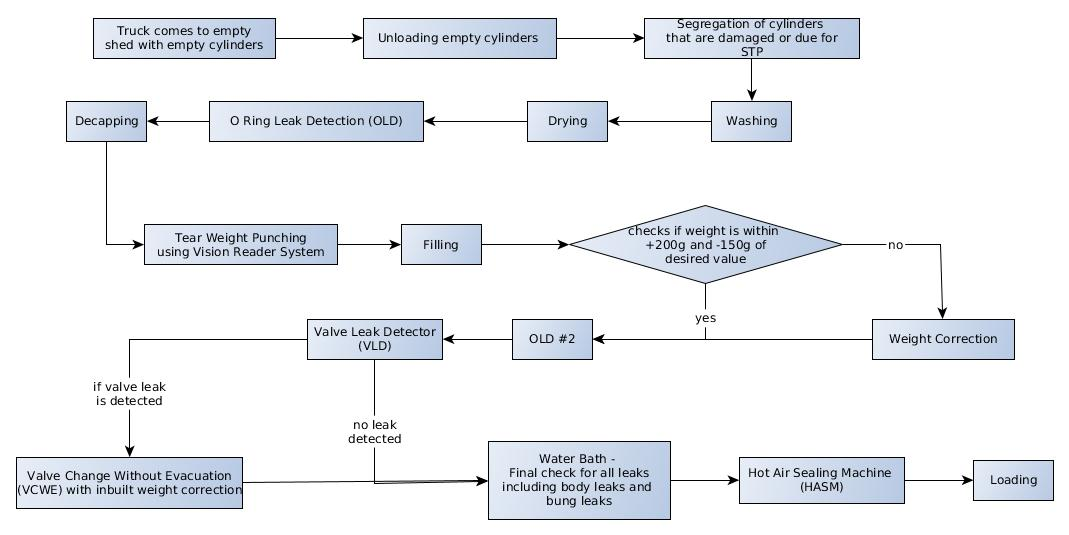
\includegraphics[width=\linewidth]{lpg_flow}
		\caption{LPG filling process flow}
		\label{lpg_flow}
	\end{figure}
		\begin{figure}[h]
		\centering
		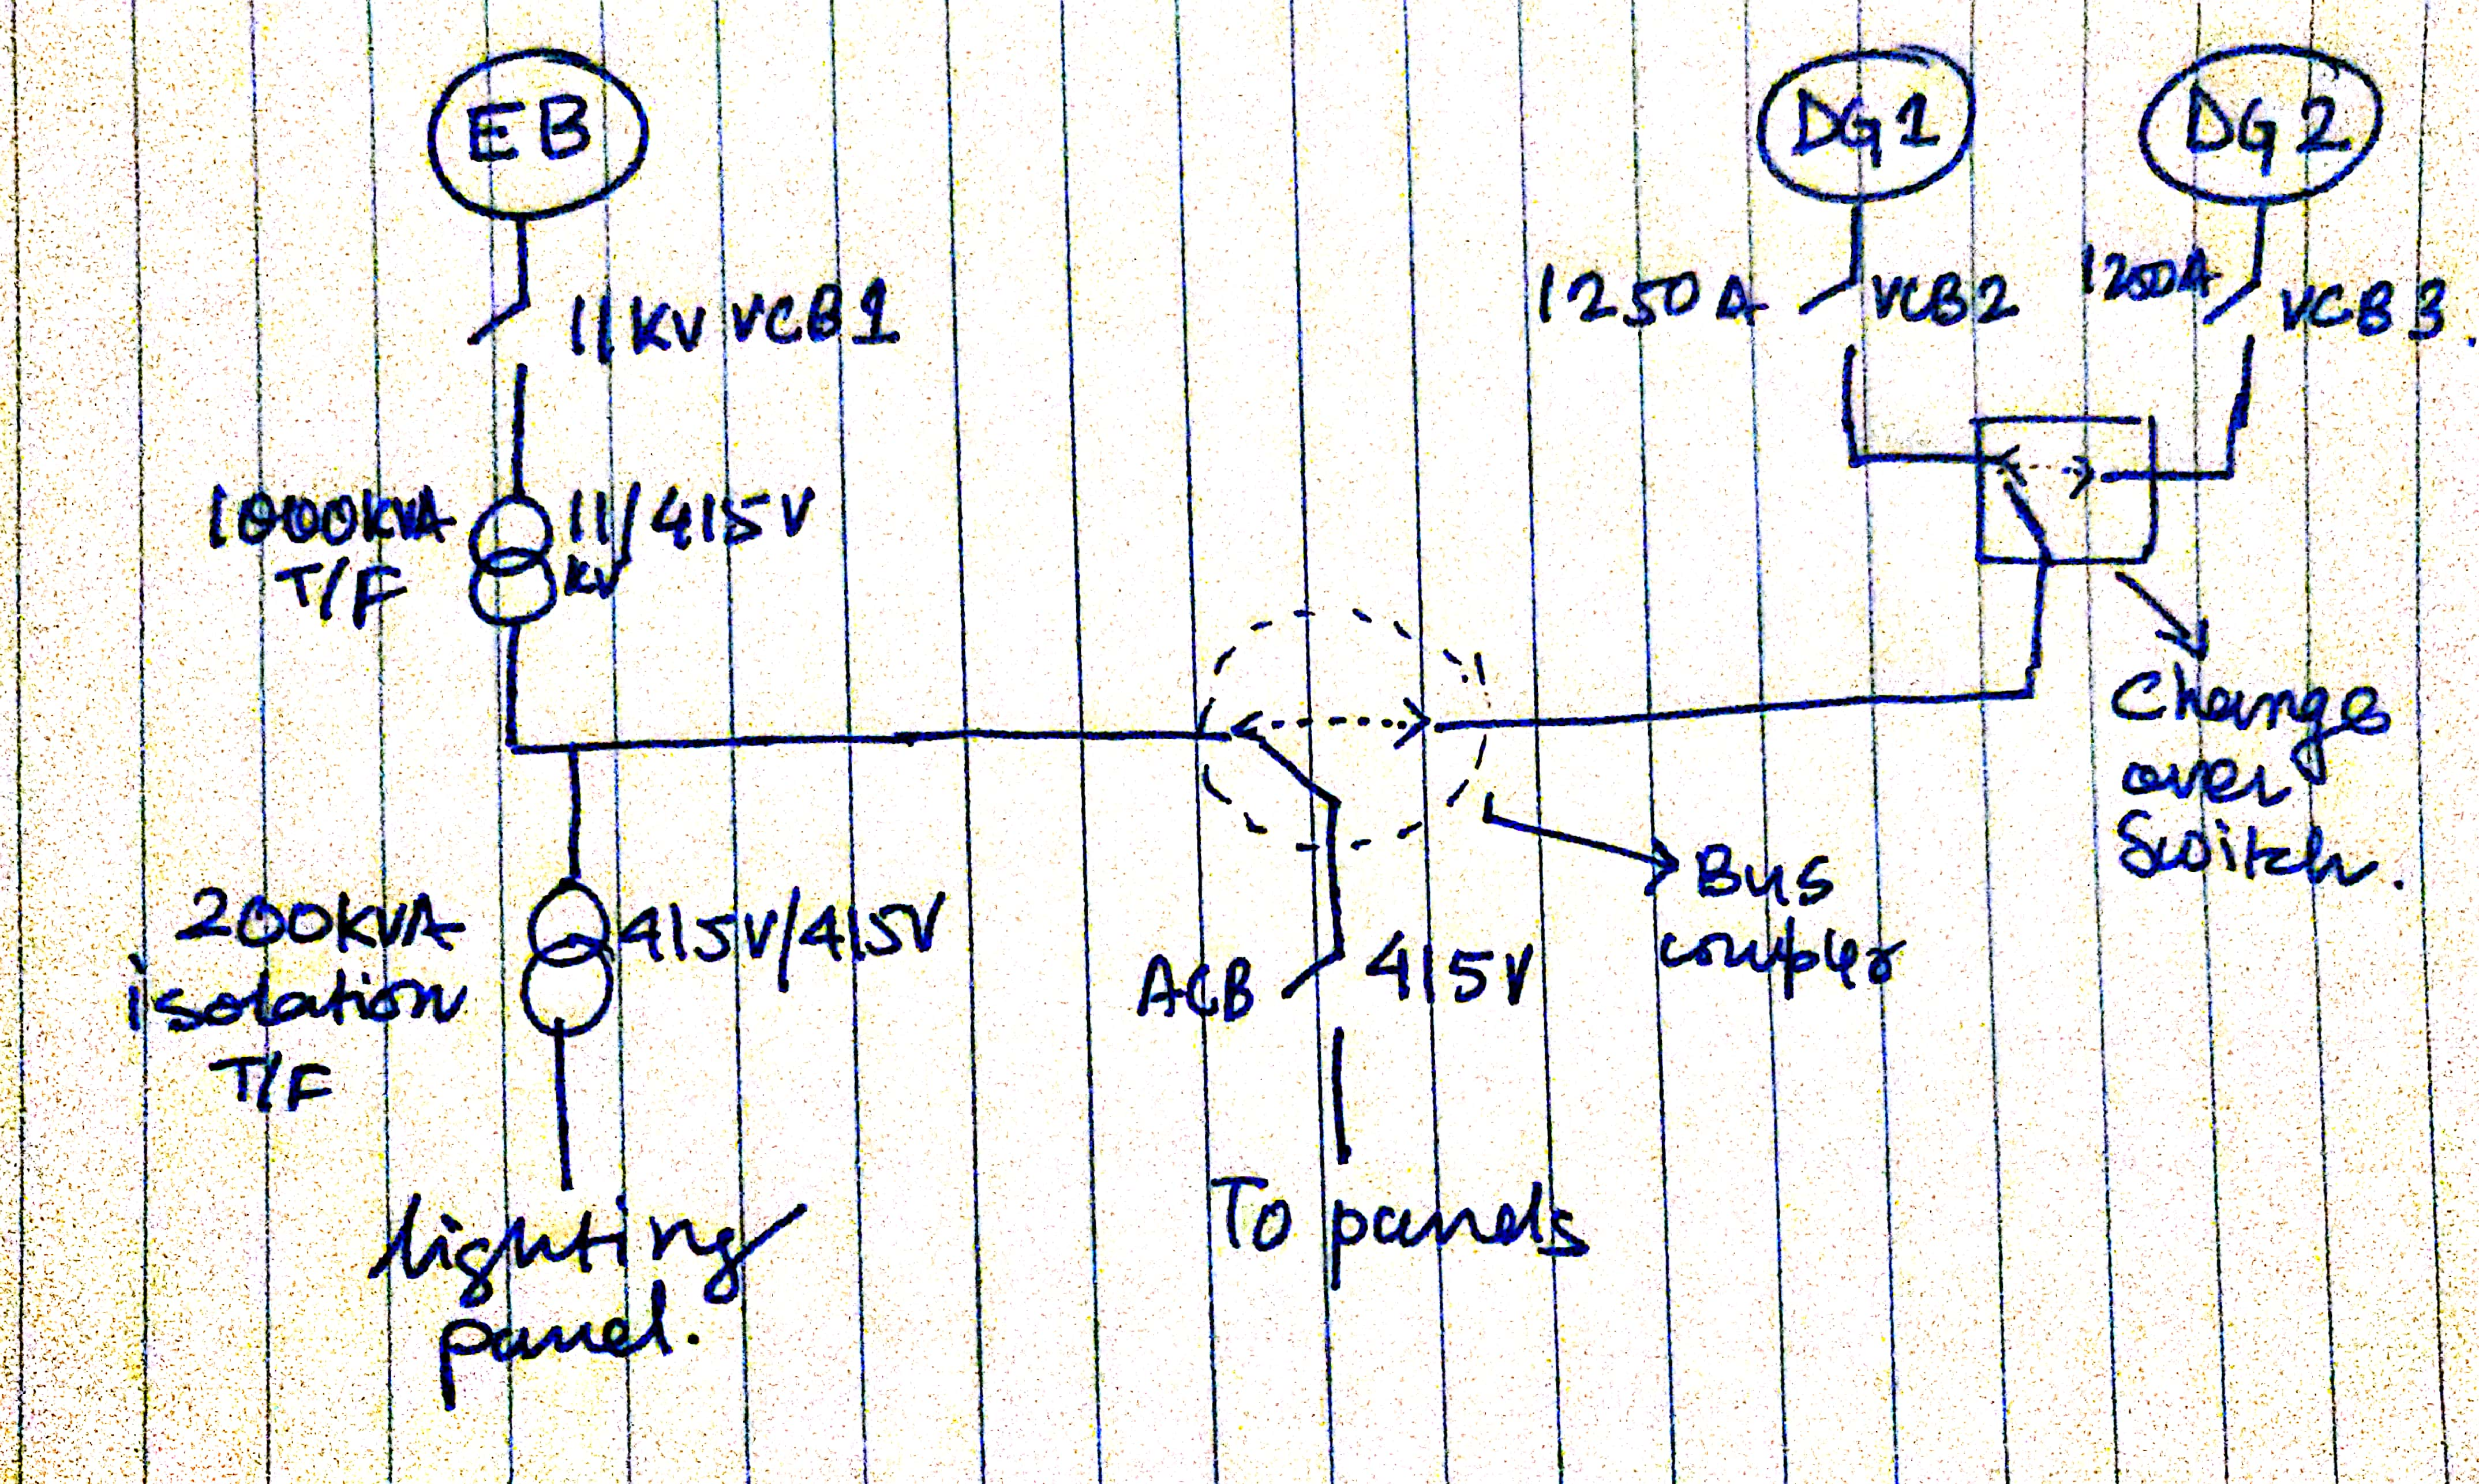
\includegraphics[width=\linewidth]{bp_singlelinediag}
		\caption{Basic single line diagram of a bottling plant electrical distribution system}
		\label{bp_singlelinediag}
	\end{figure}
	\begin{figure}[h]
		\centering
		\subfloat[][Schematic diagram of a Switch Fuse Unit]{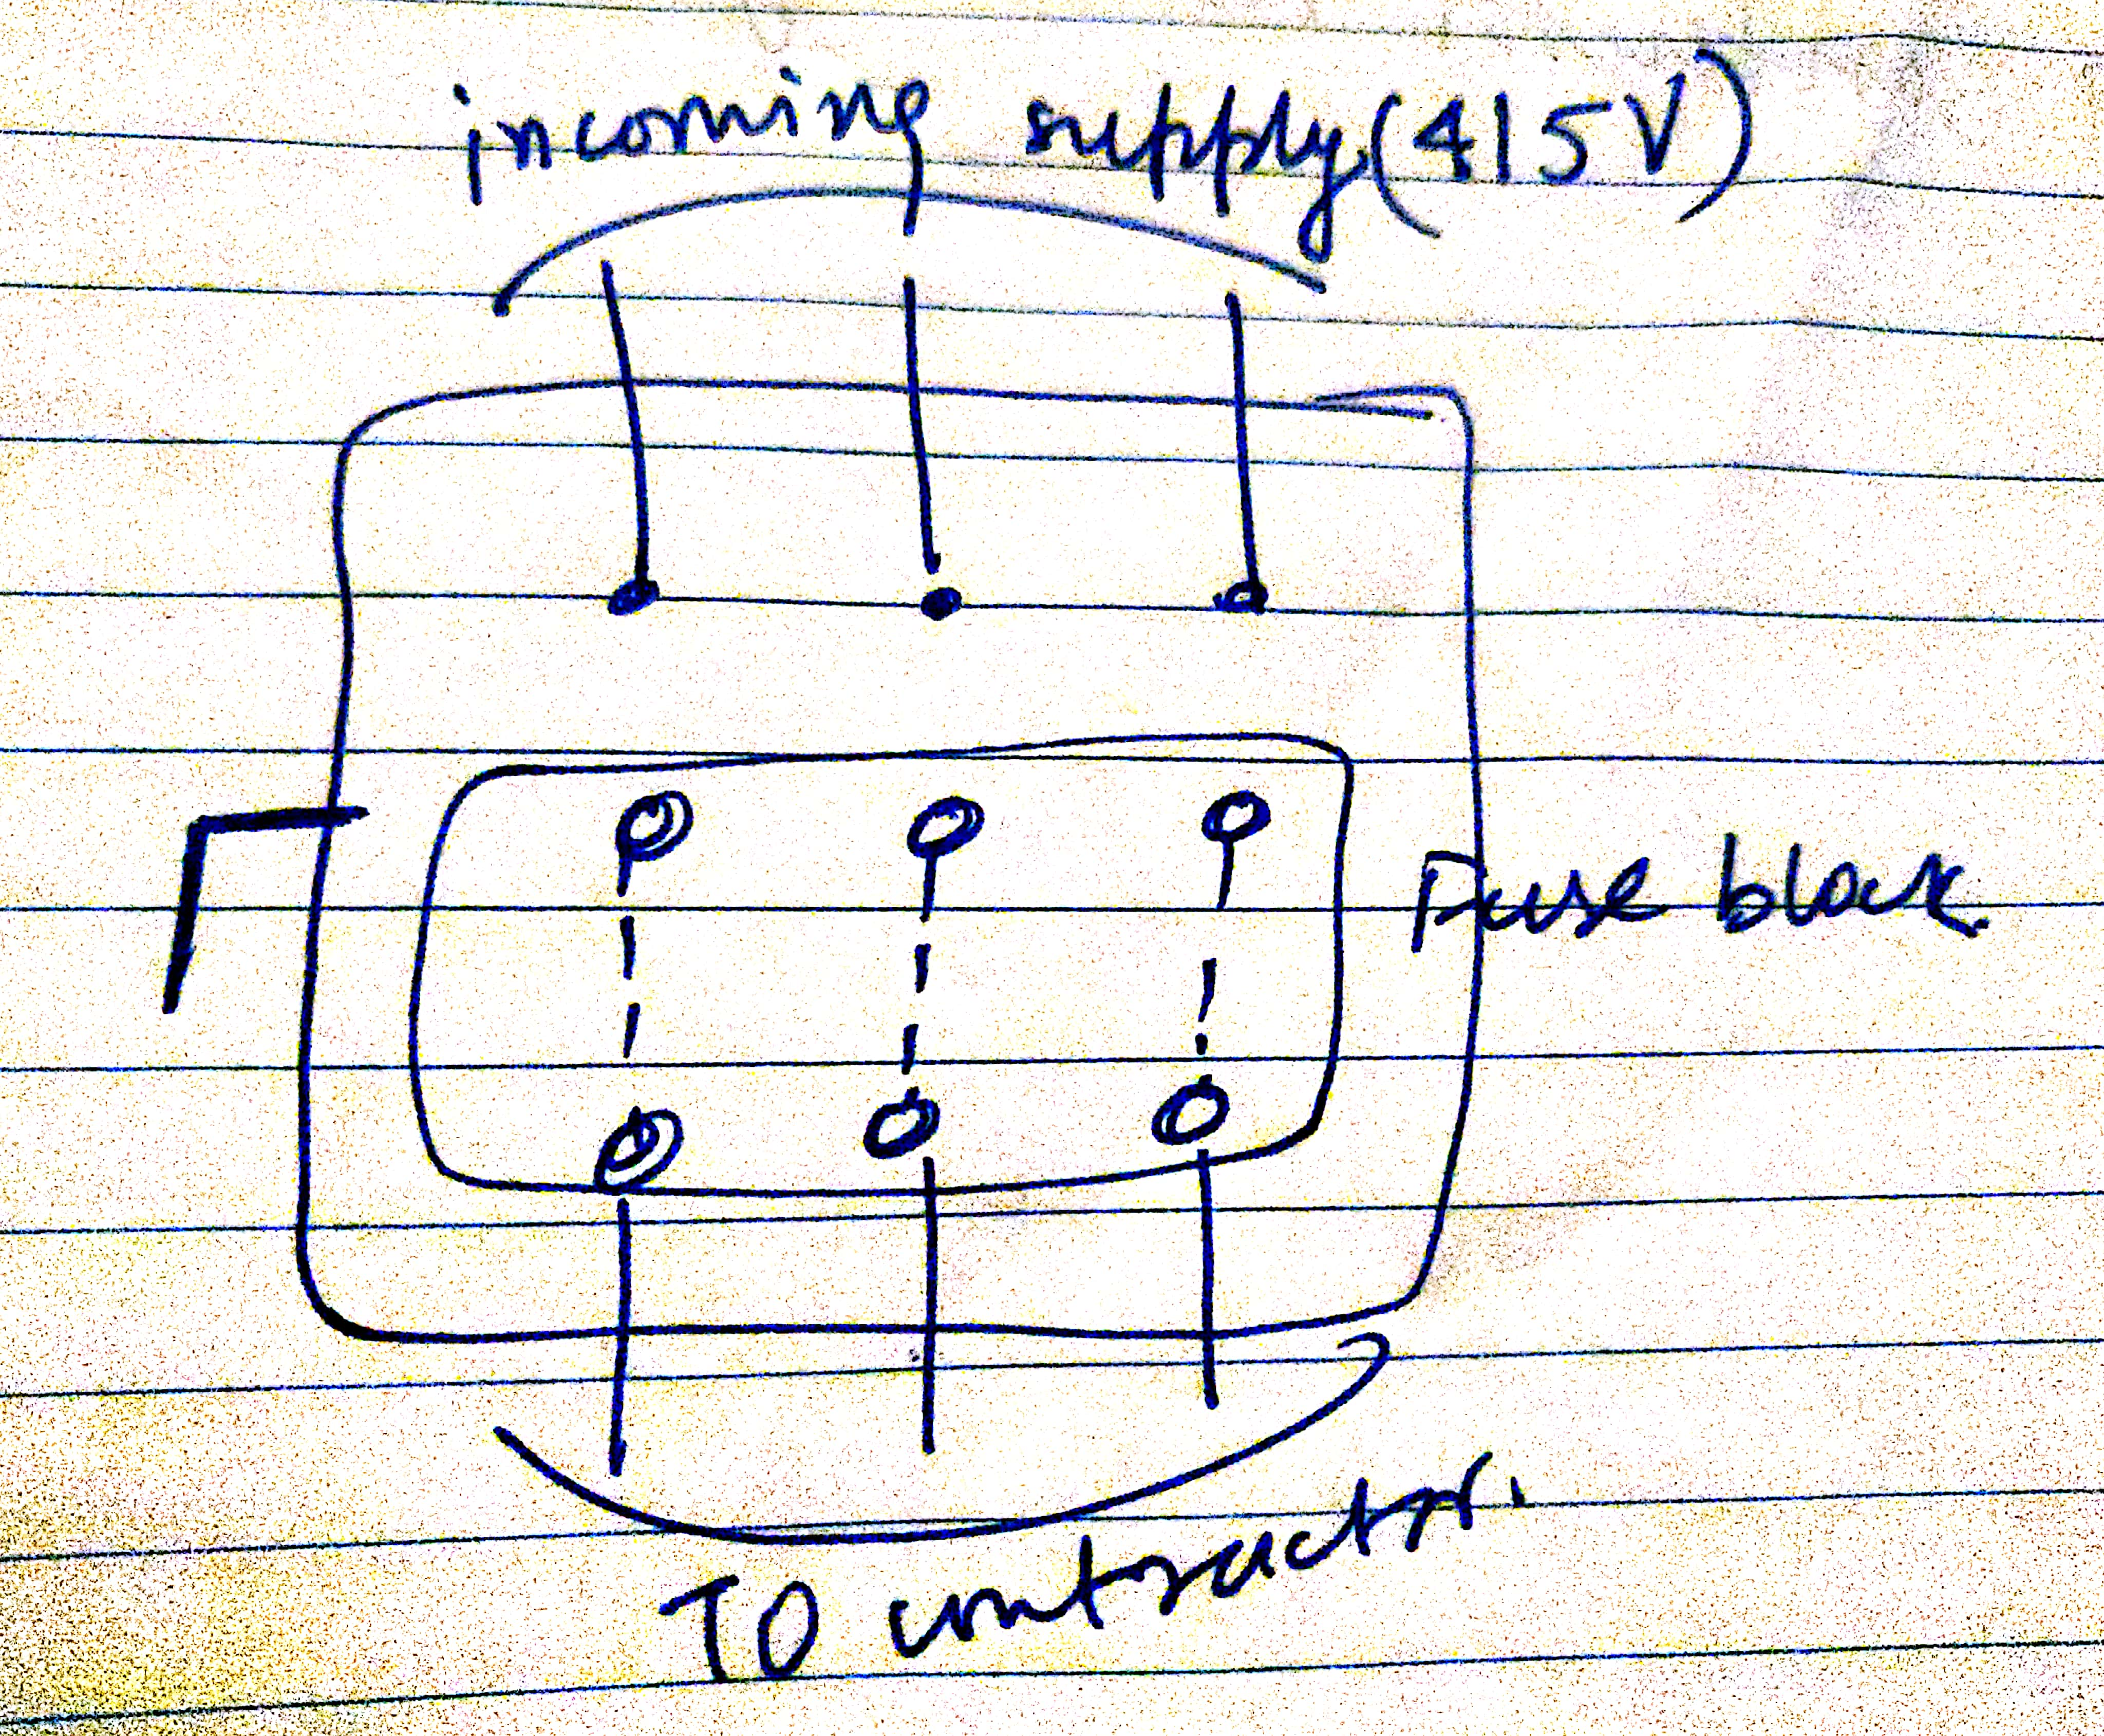
\includegraphics[width=0.5\linewidth]{sfu}\label{sfu}}
		\subfloat[][Inside view of a panel showing its safety features]{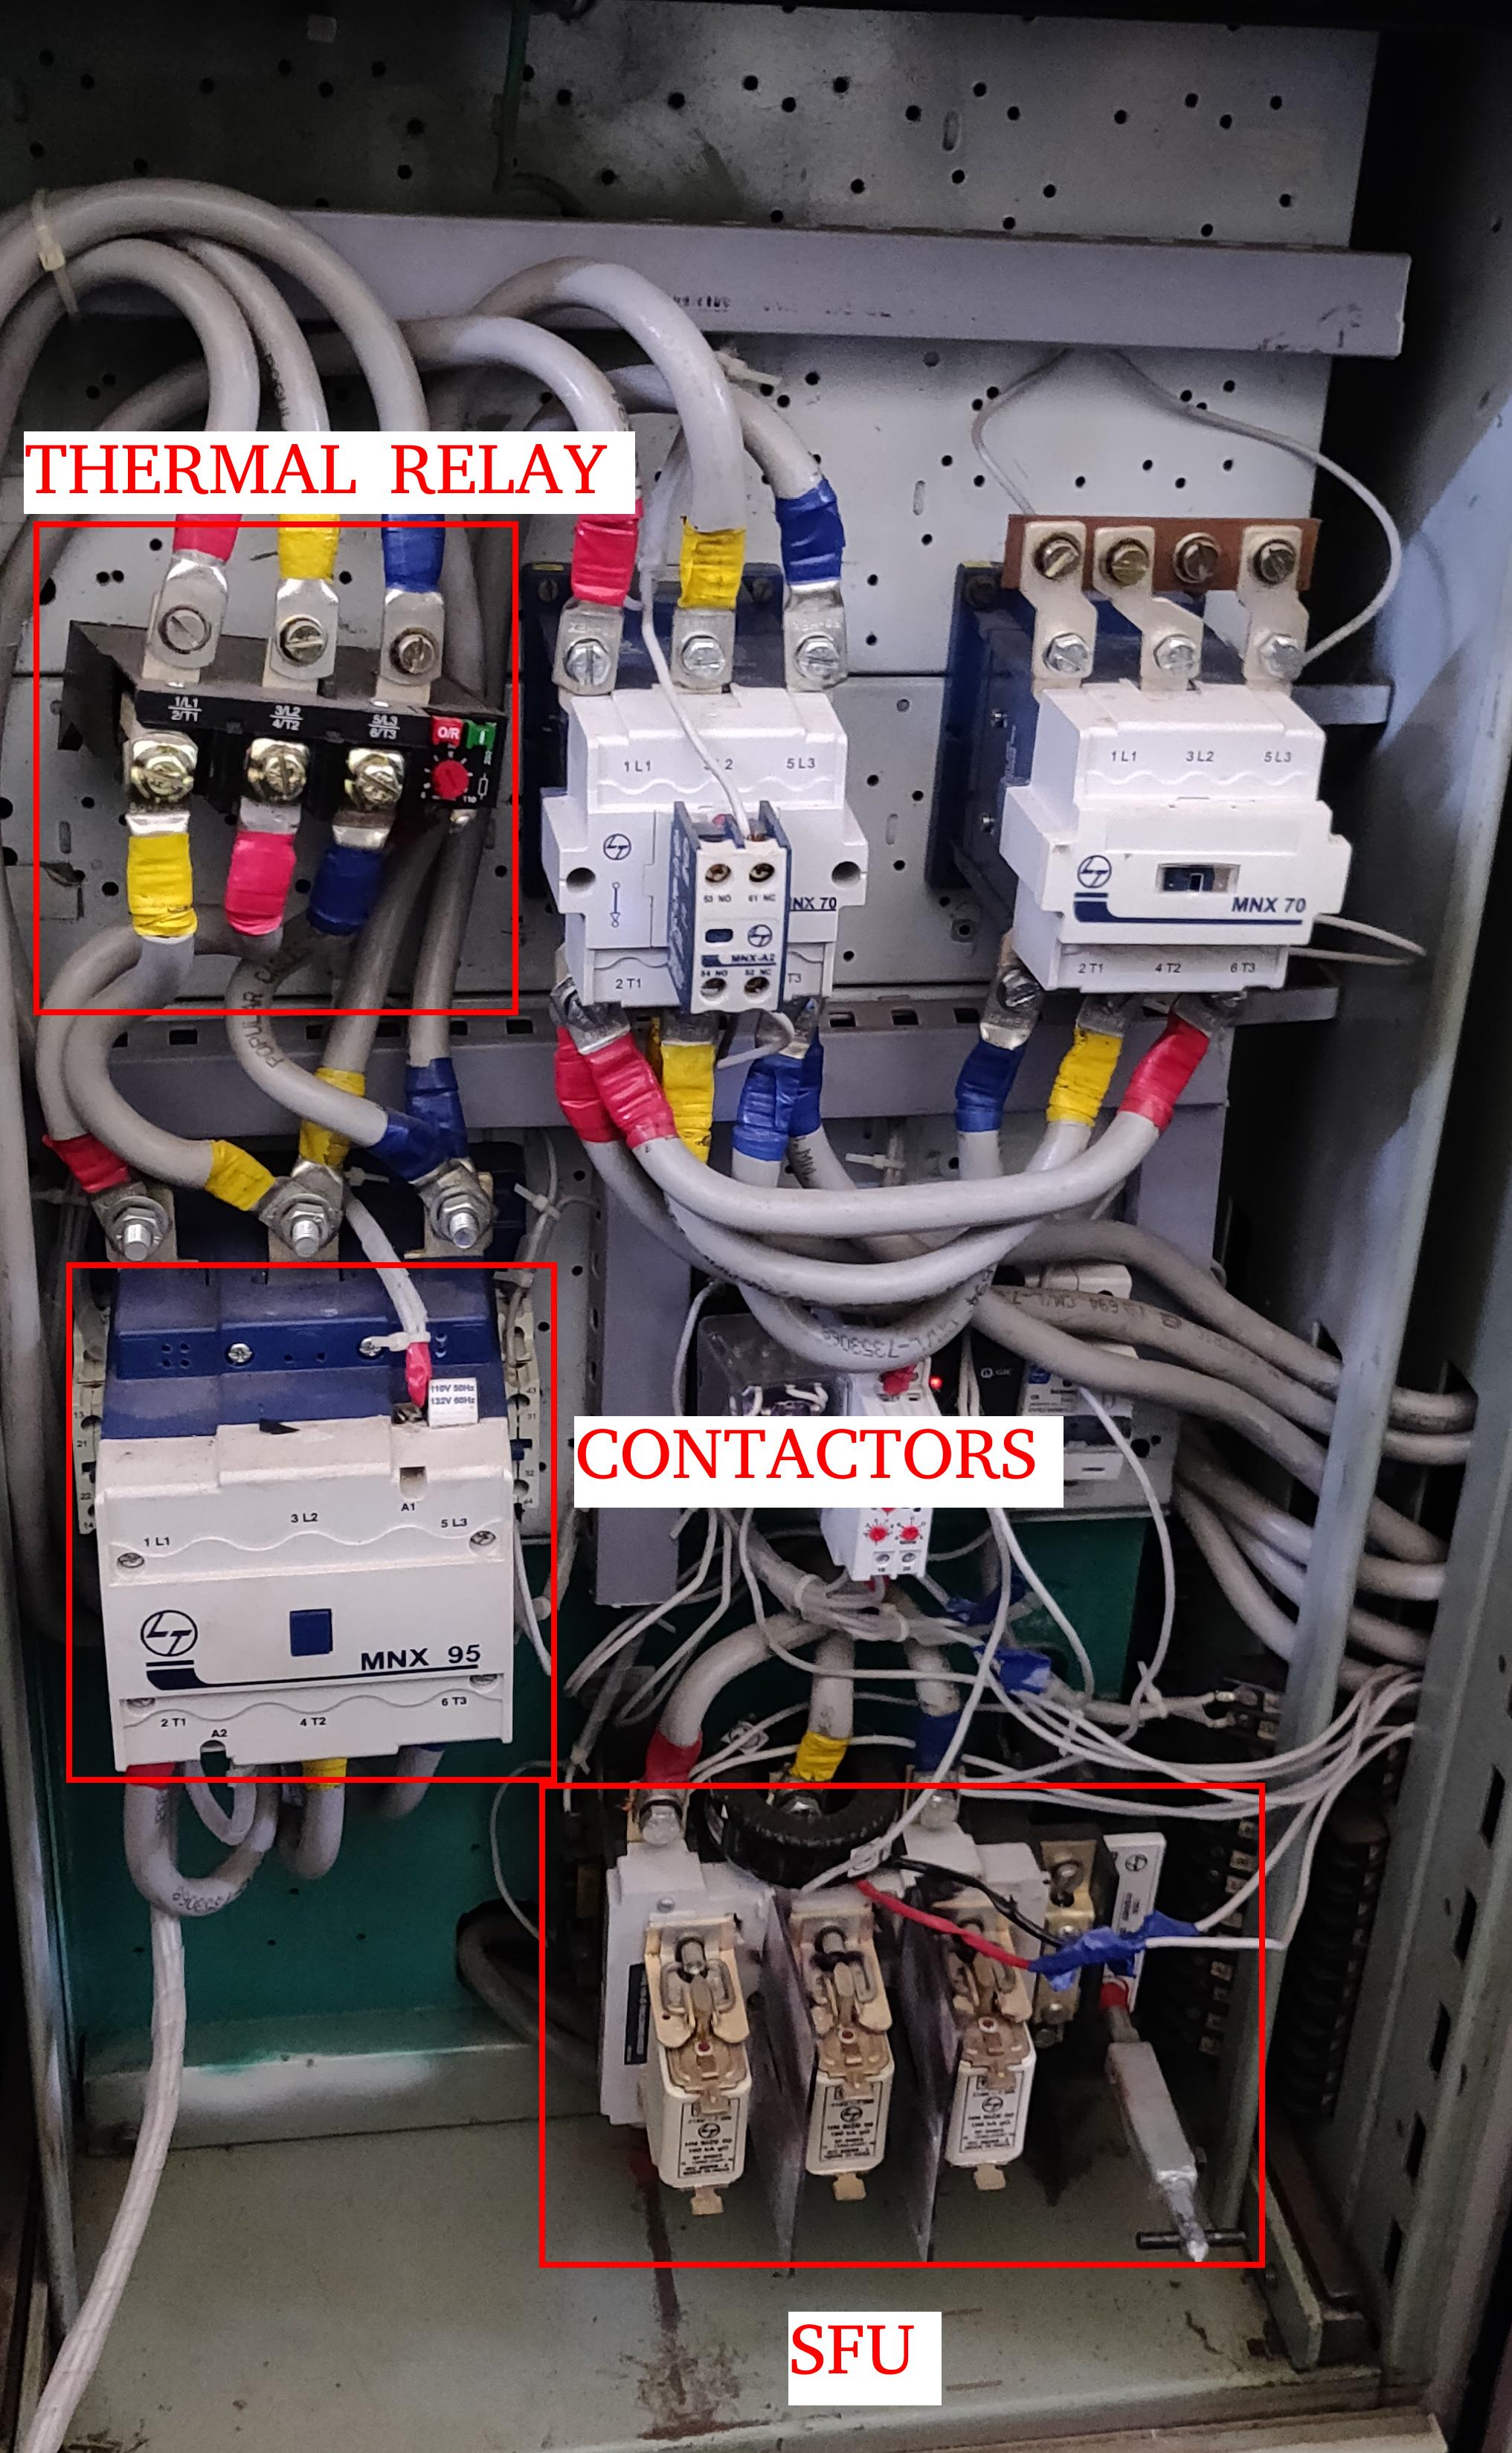
\includegraphics[height=10cm,width=0.5\linewidth]{inside_panel}\label{inside_panel}}
		\caption{Theoretical and real panel equipment protection apparatus}
		\label{bp_panel}
	\end{figure}
	\begin{figure}[h]
		\centering
		\subfloat[Schematic diagram of the dc power delivery system]{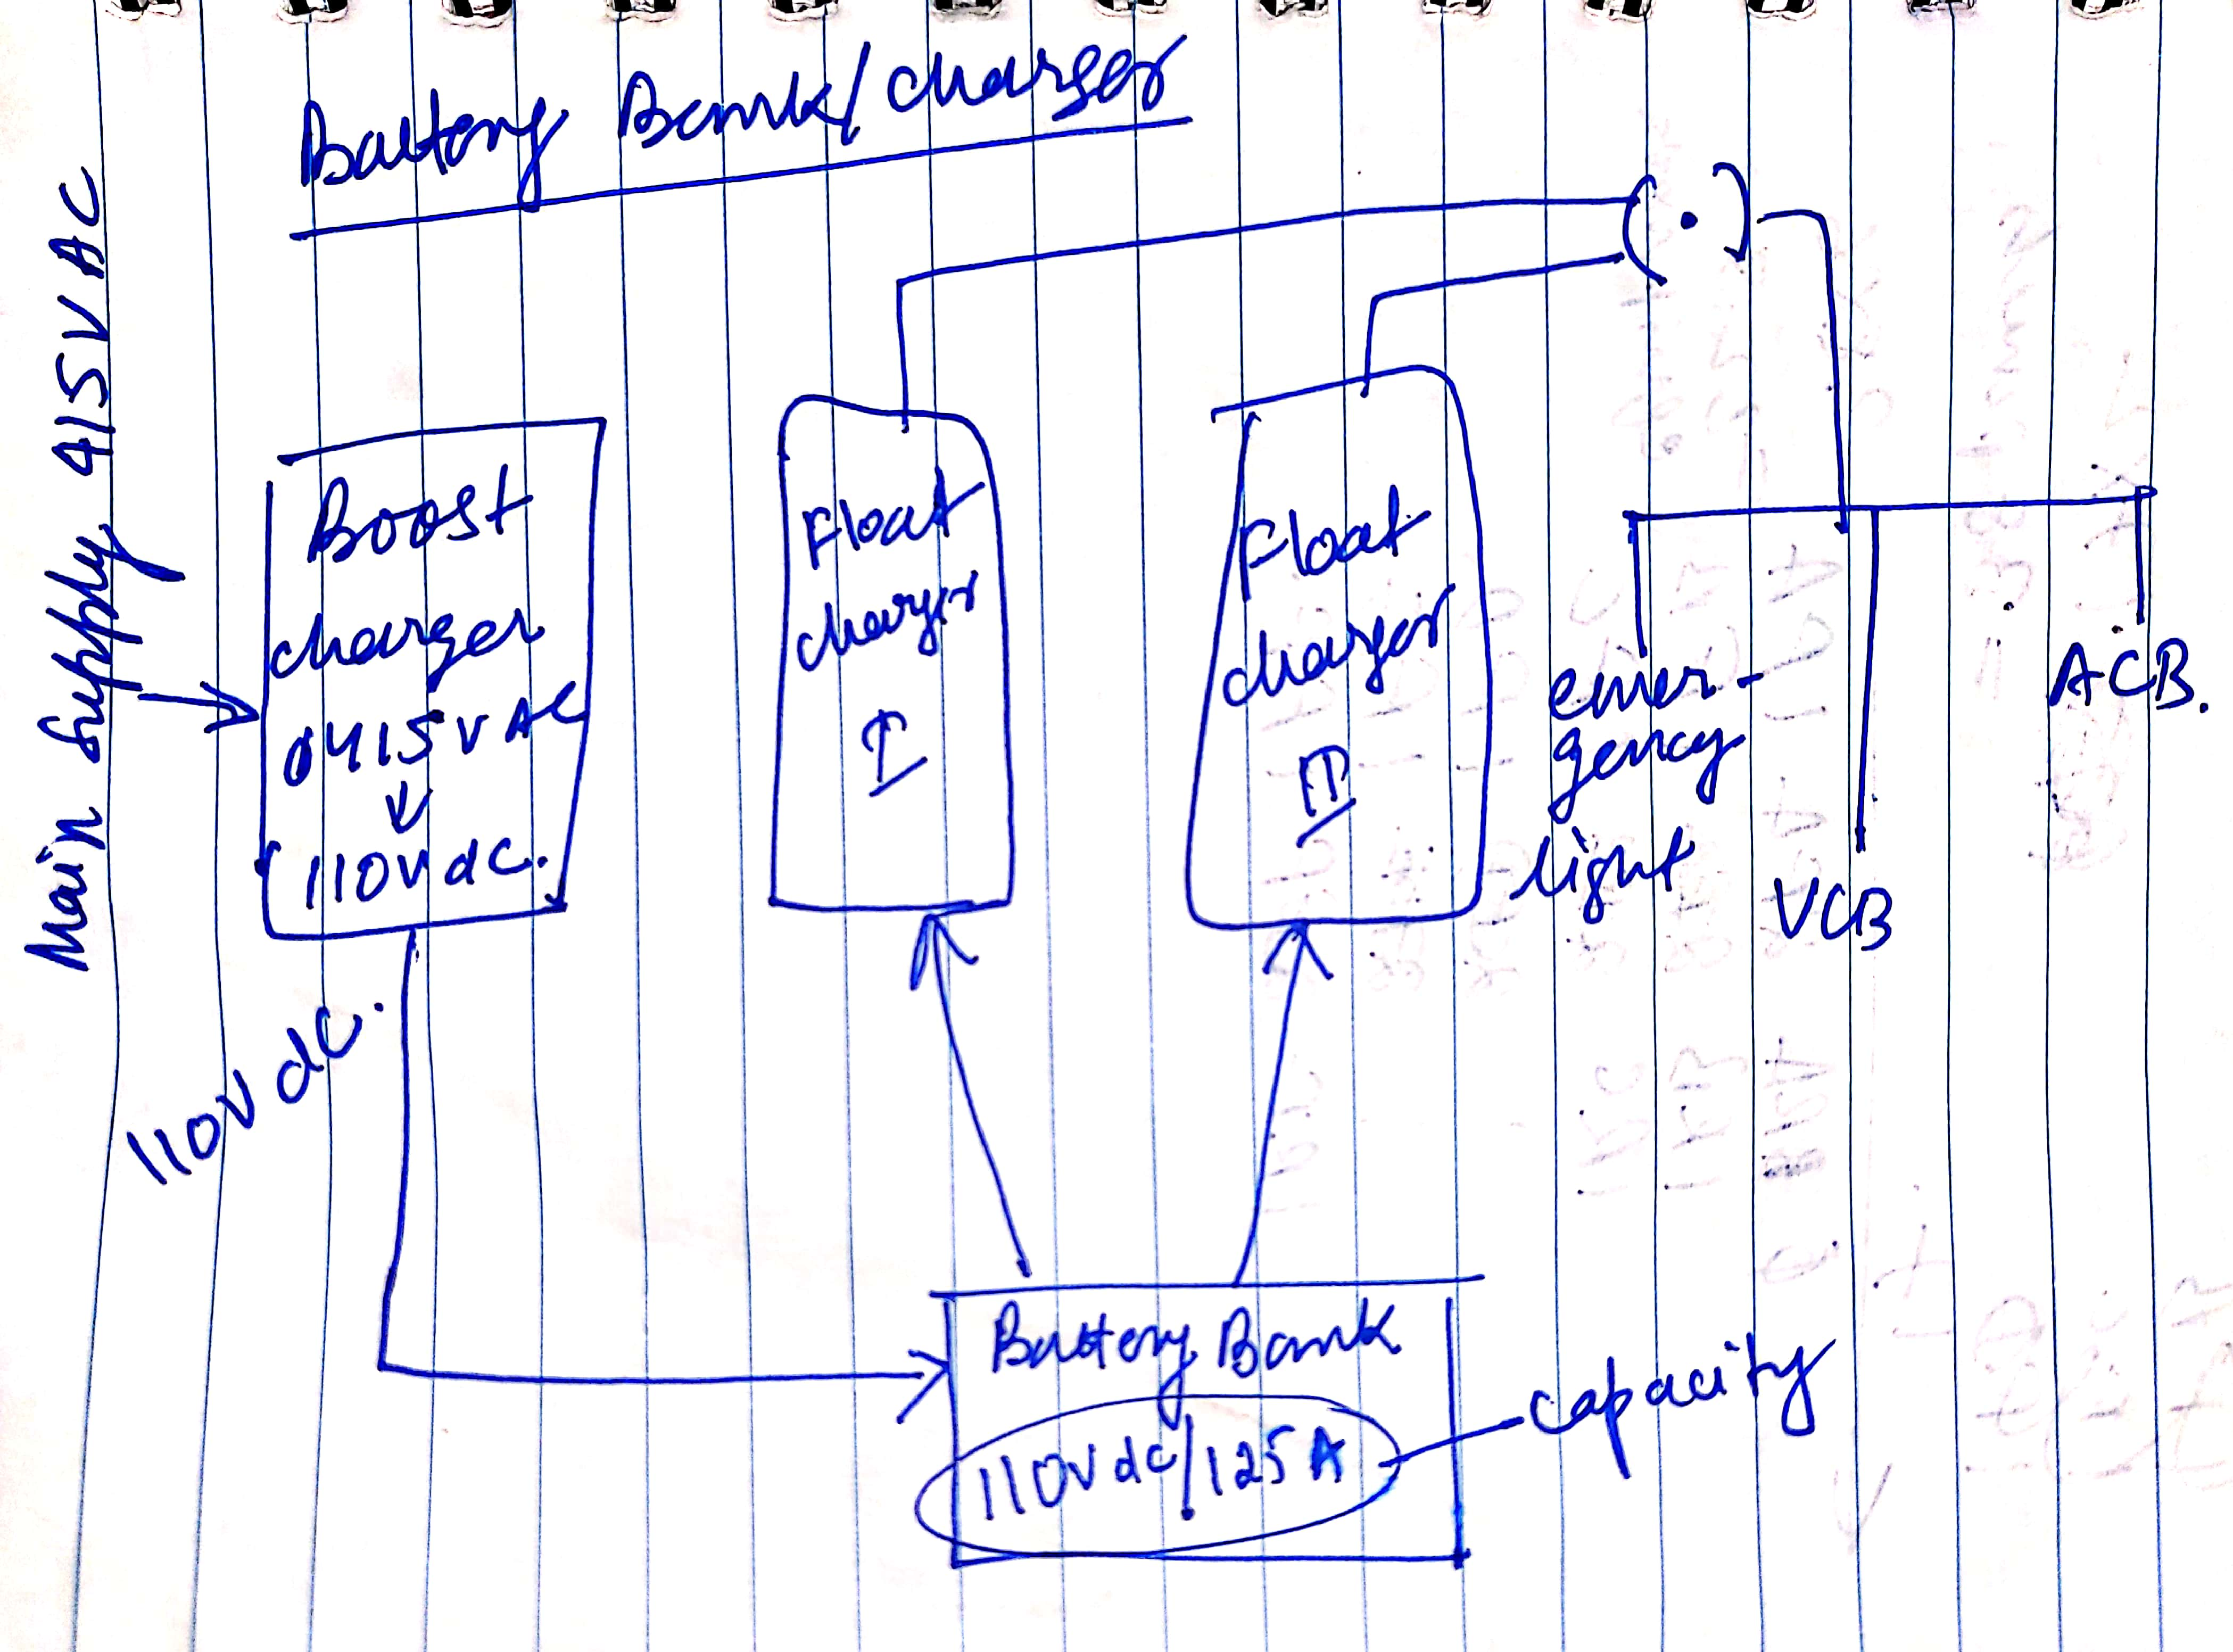
\includegraphics[width=0.5\linewidth]{dc_distribution}\label{dc_distribution}}
		\subfloat[Schematic diagram of the dc power delivery system]{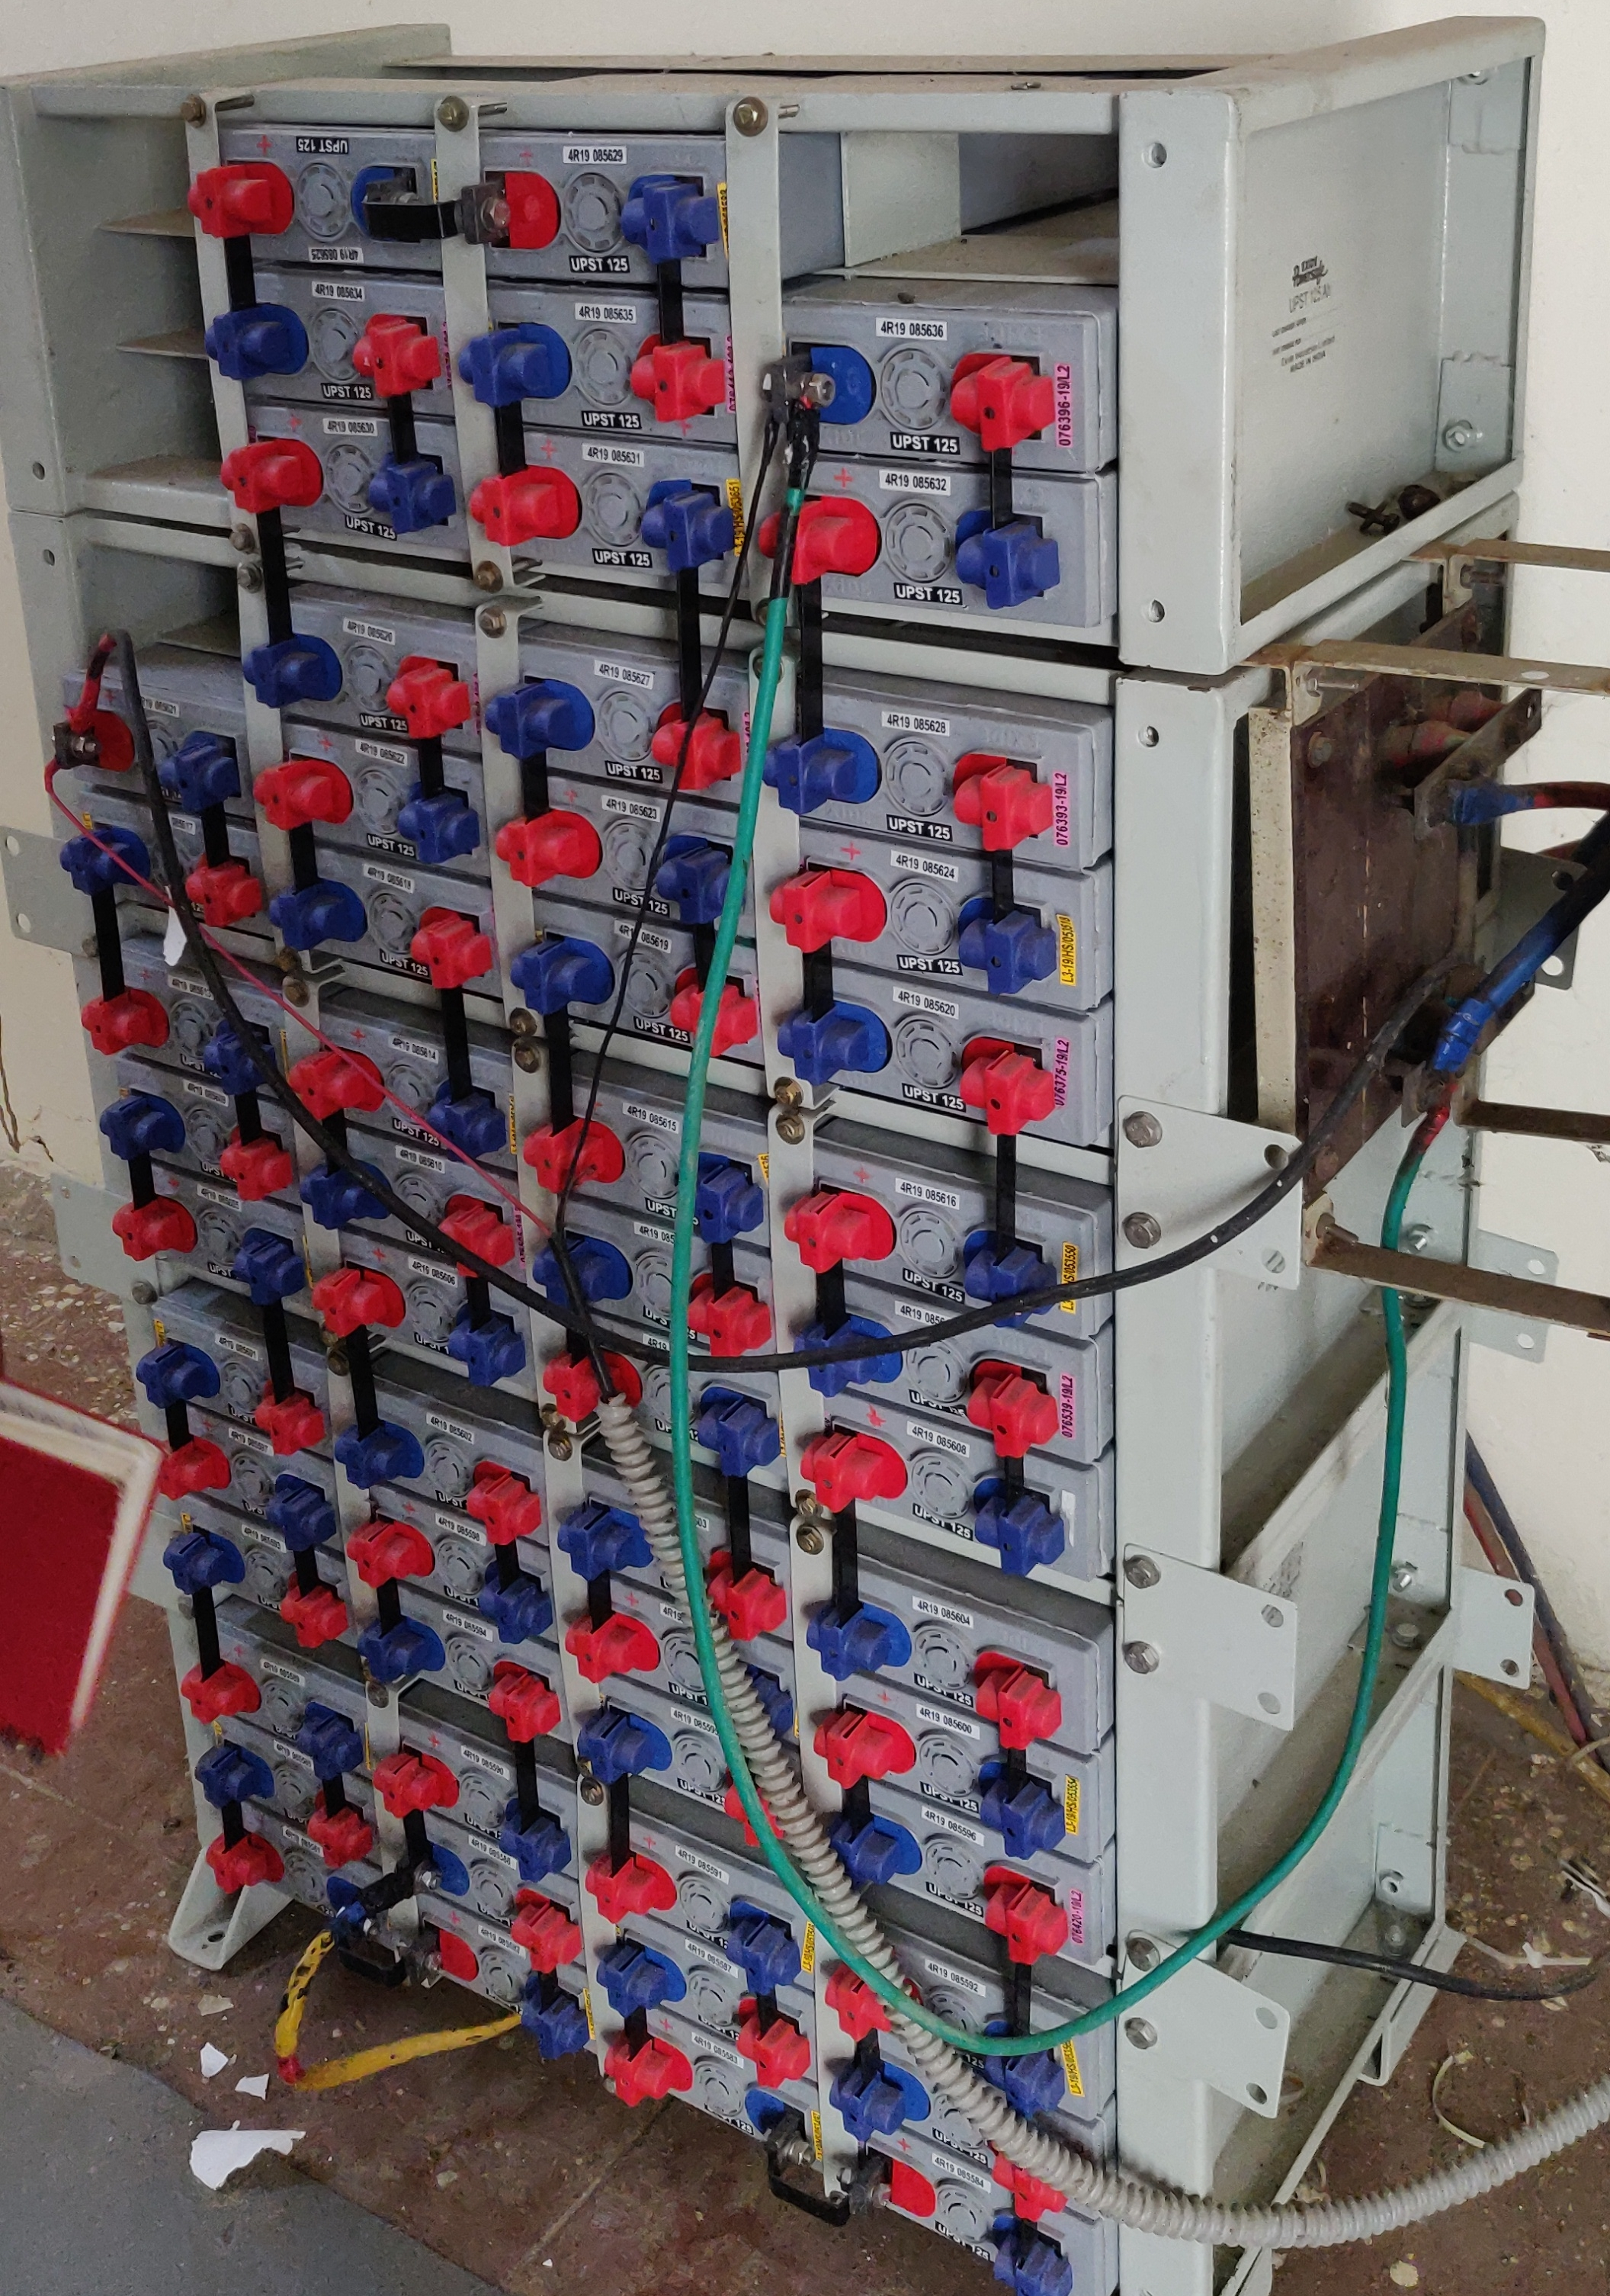
\includegraphics[height=10cm]{battery_pack_sanand}\label{battery_pack_sanand}}
		\caption{DC power delivery system}
		\label{dc_power_sanand}
	\end{figure}
	\begin{figure}[h]
		\centering
		\subfloat[][Neutral Earthing]{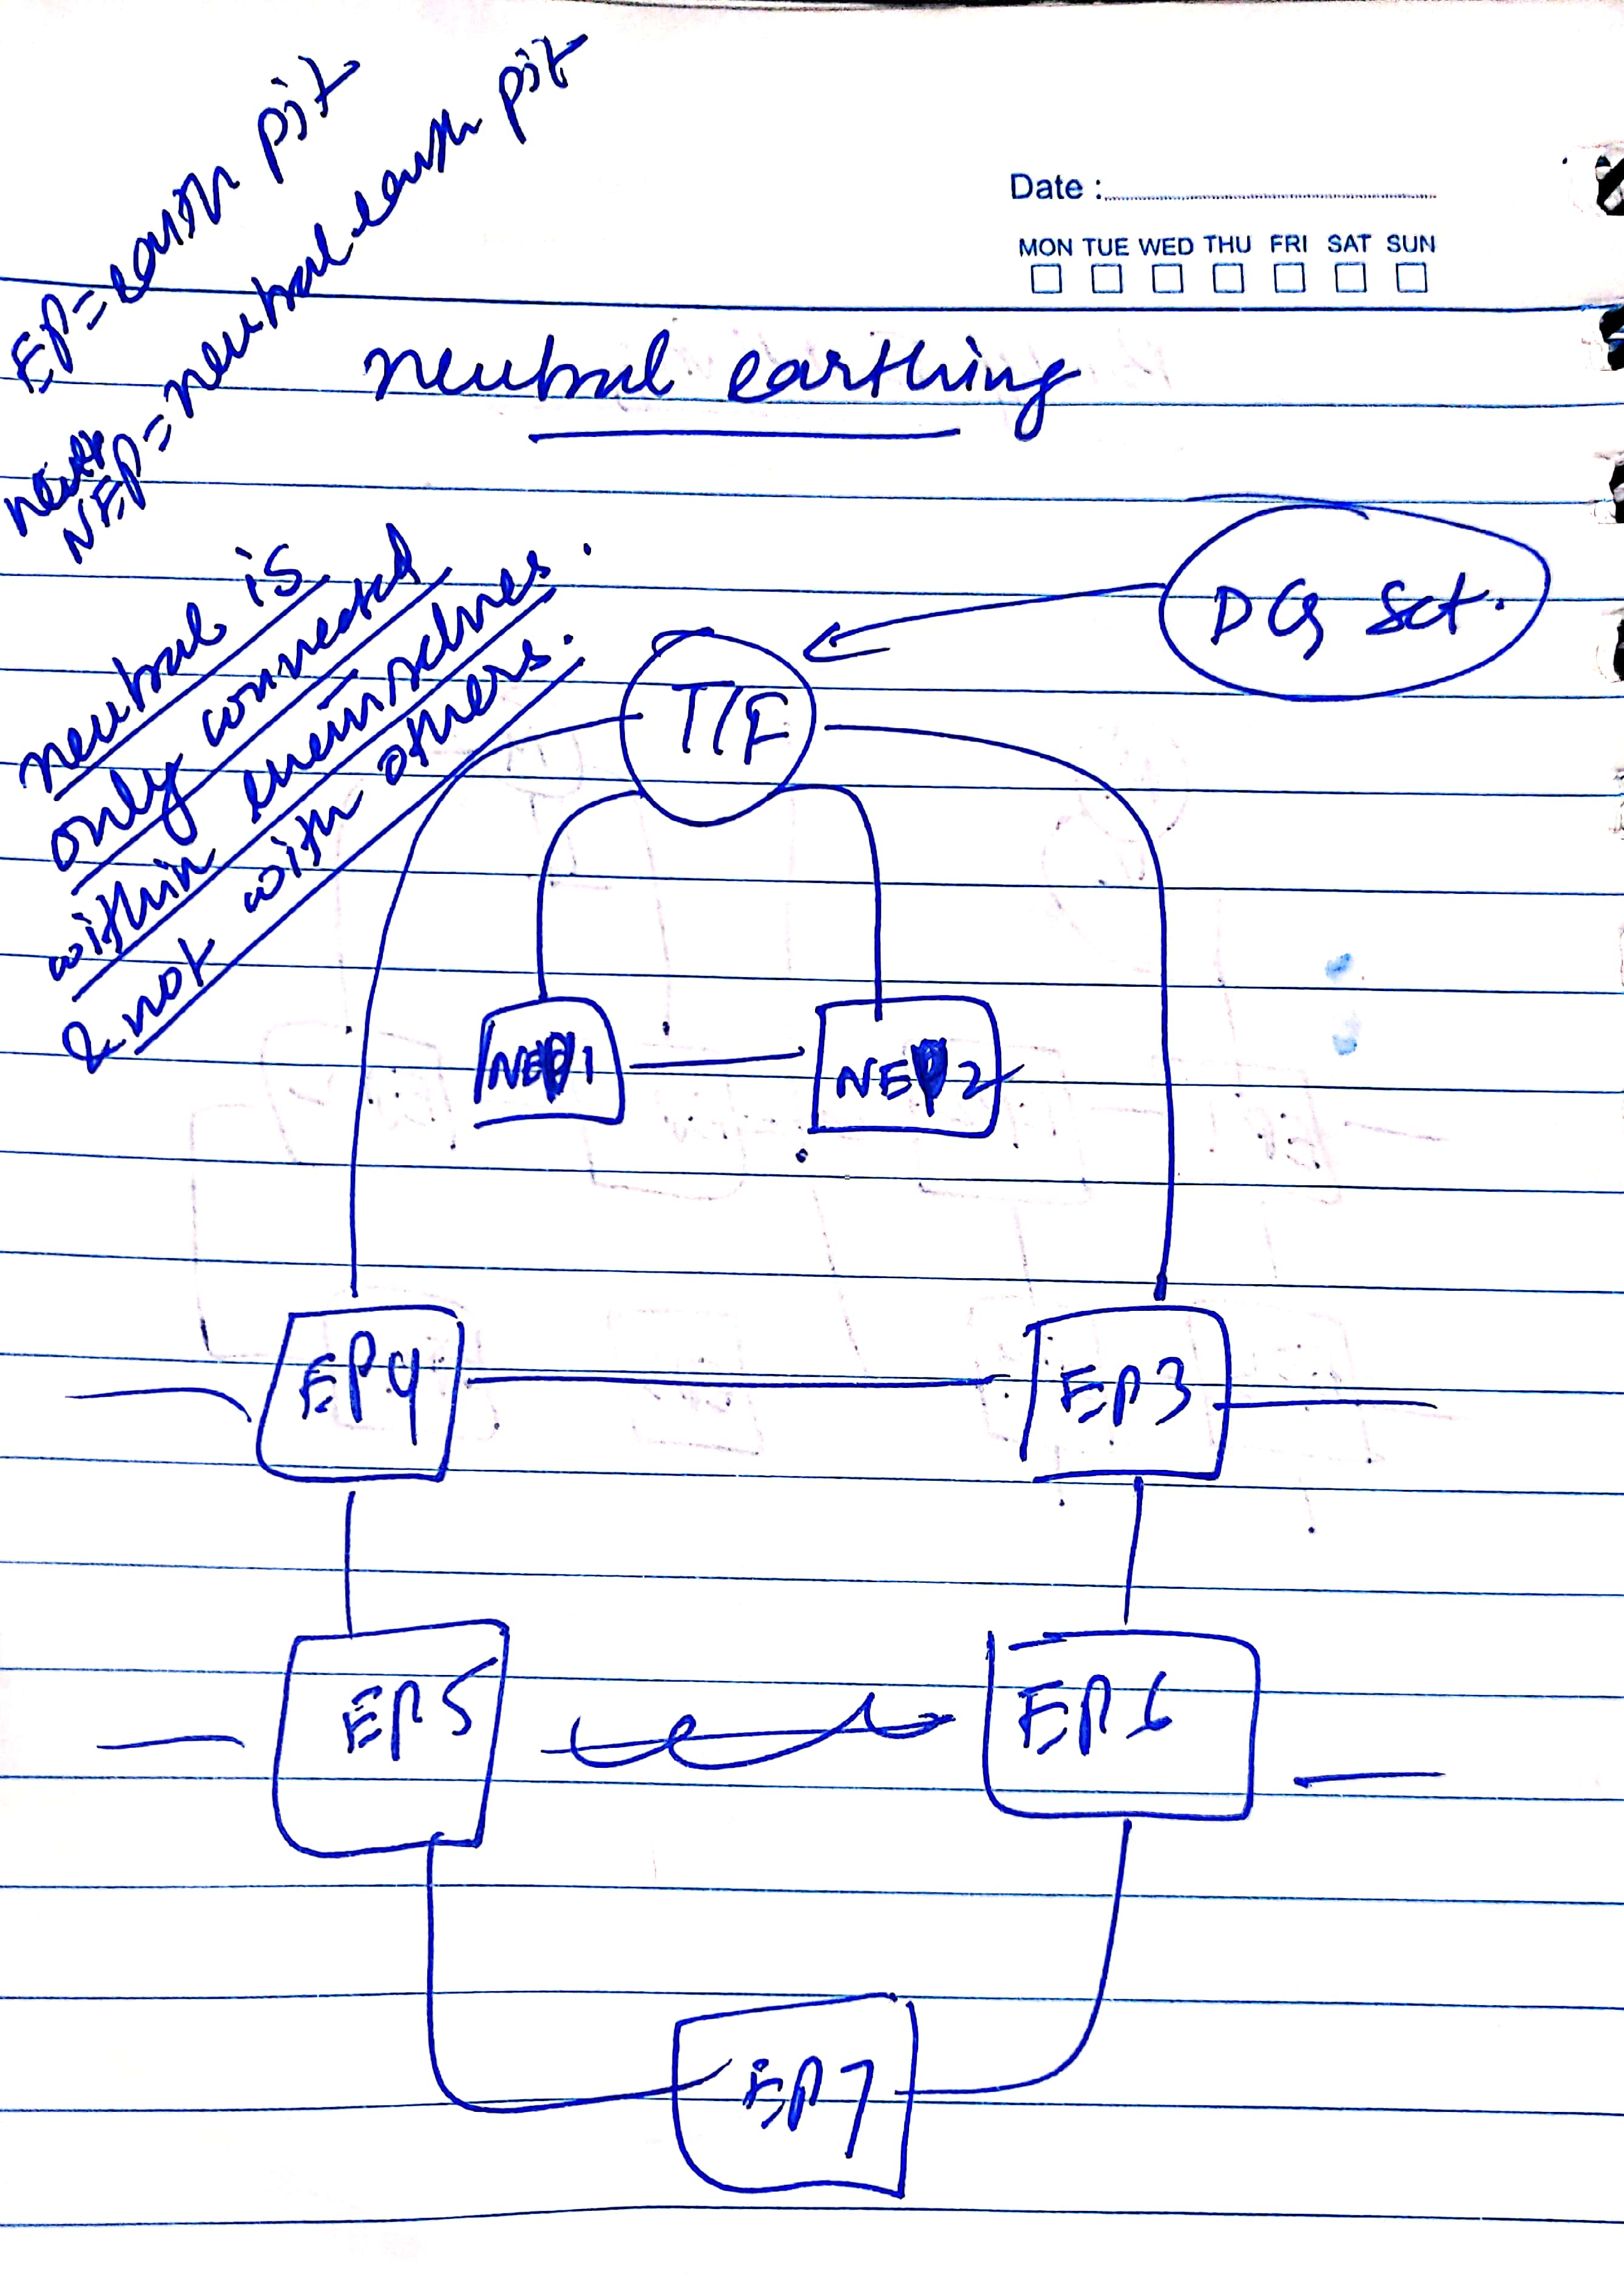
\includegraphics[height=10cm,width=0.33\linewidth]{neutral_earthing}\label{neutral_earthing}}
		\subfloat[][Lightning Earthing]{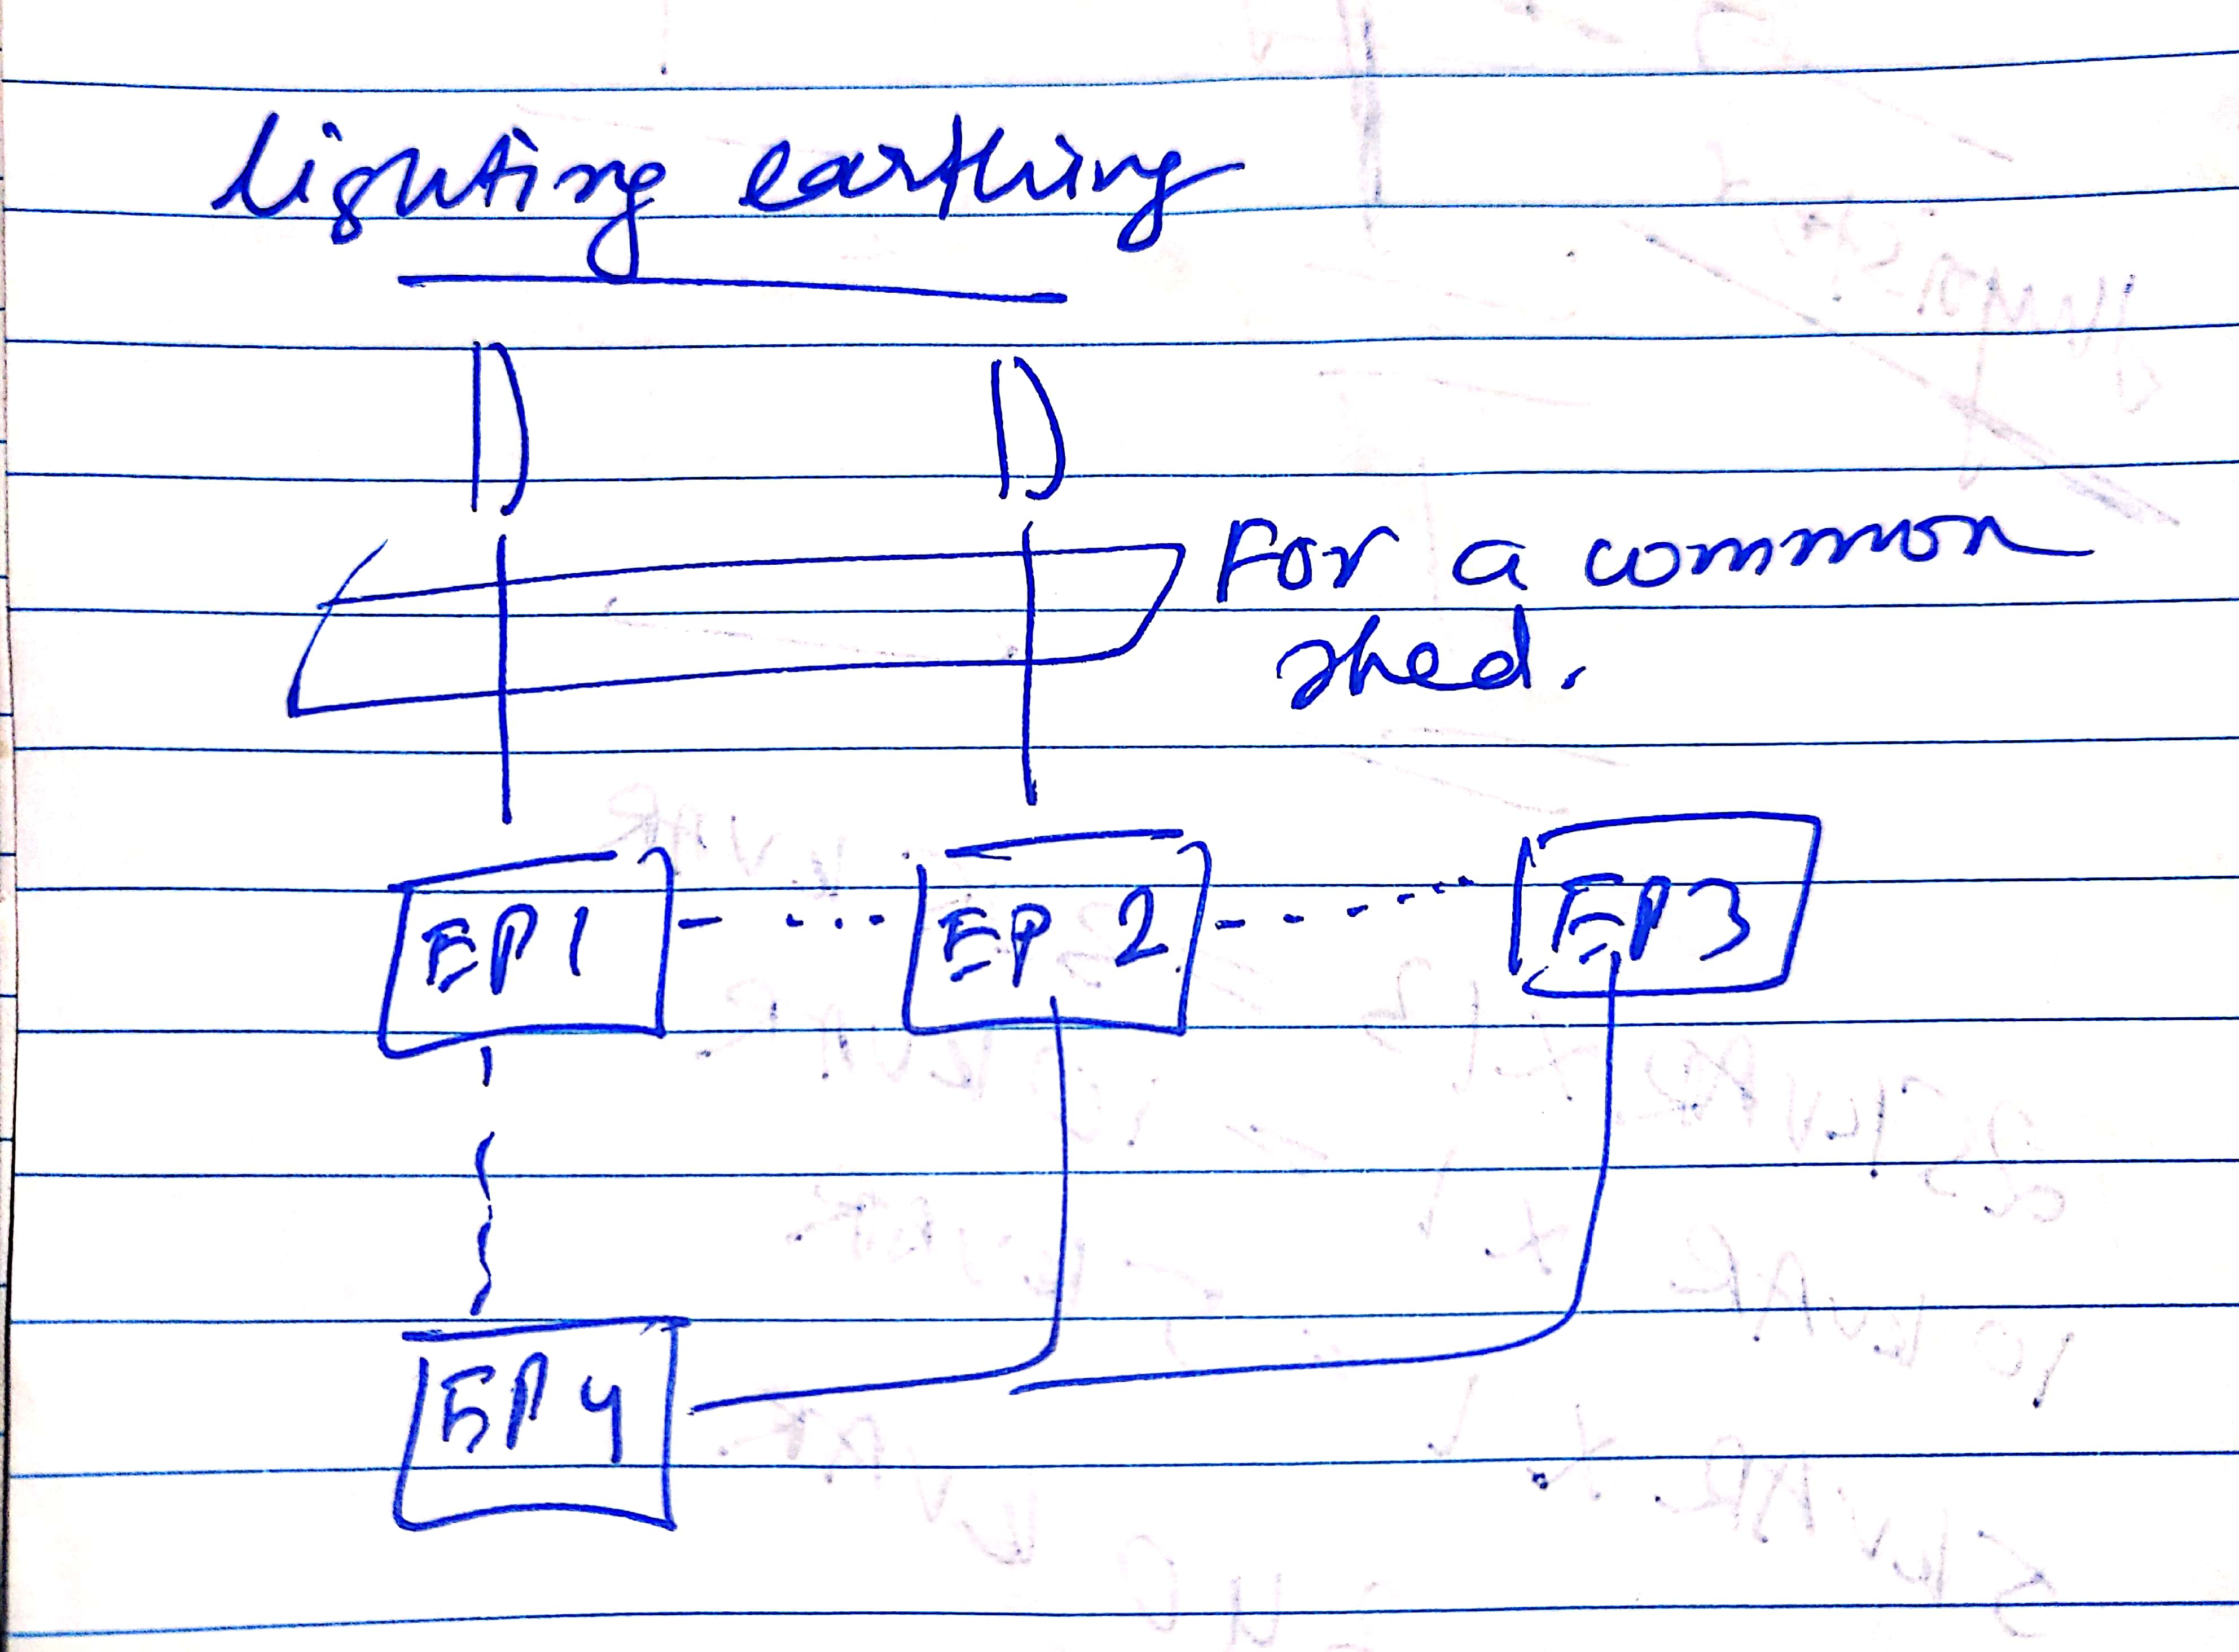
\includegraphics[height=10cm,width=0.33\linewidth]{lightning_earthing}\label{lightning_earthing}}
		\subfloat[][Body Earthing]{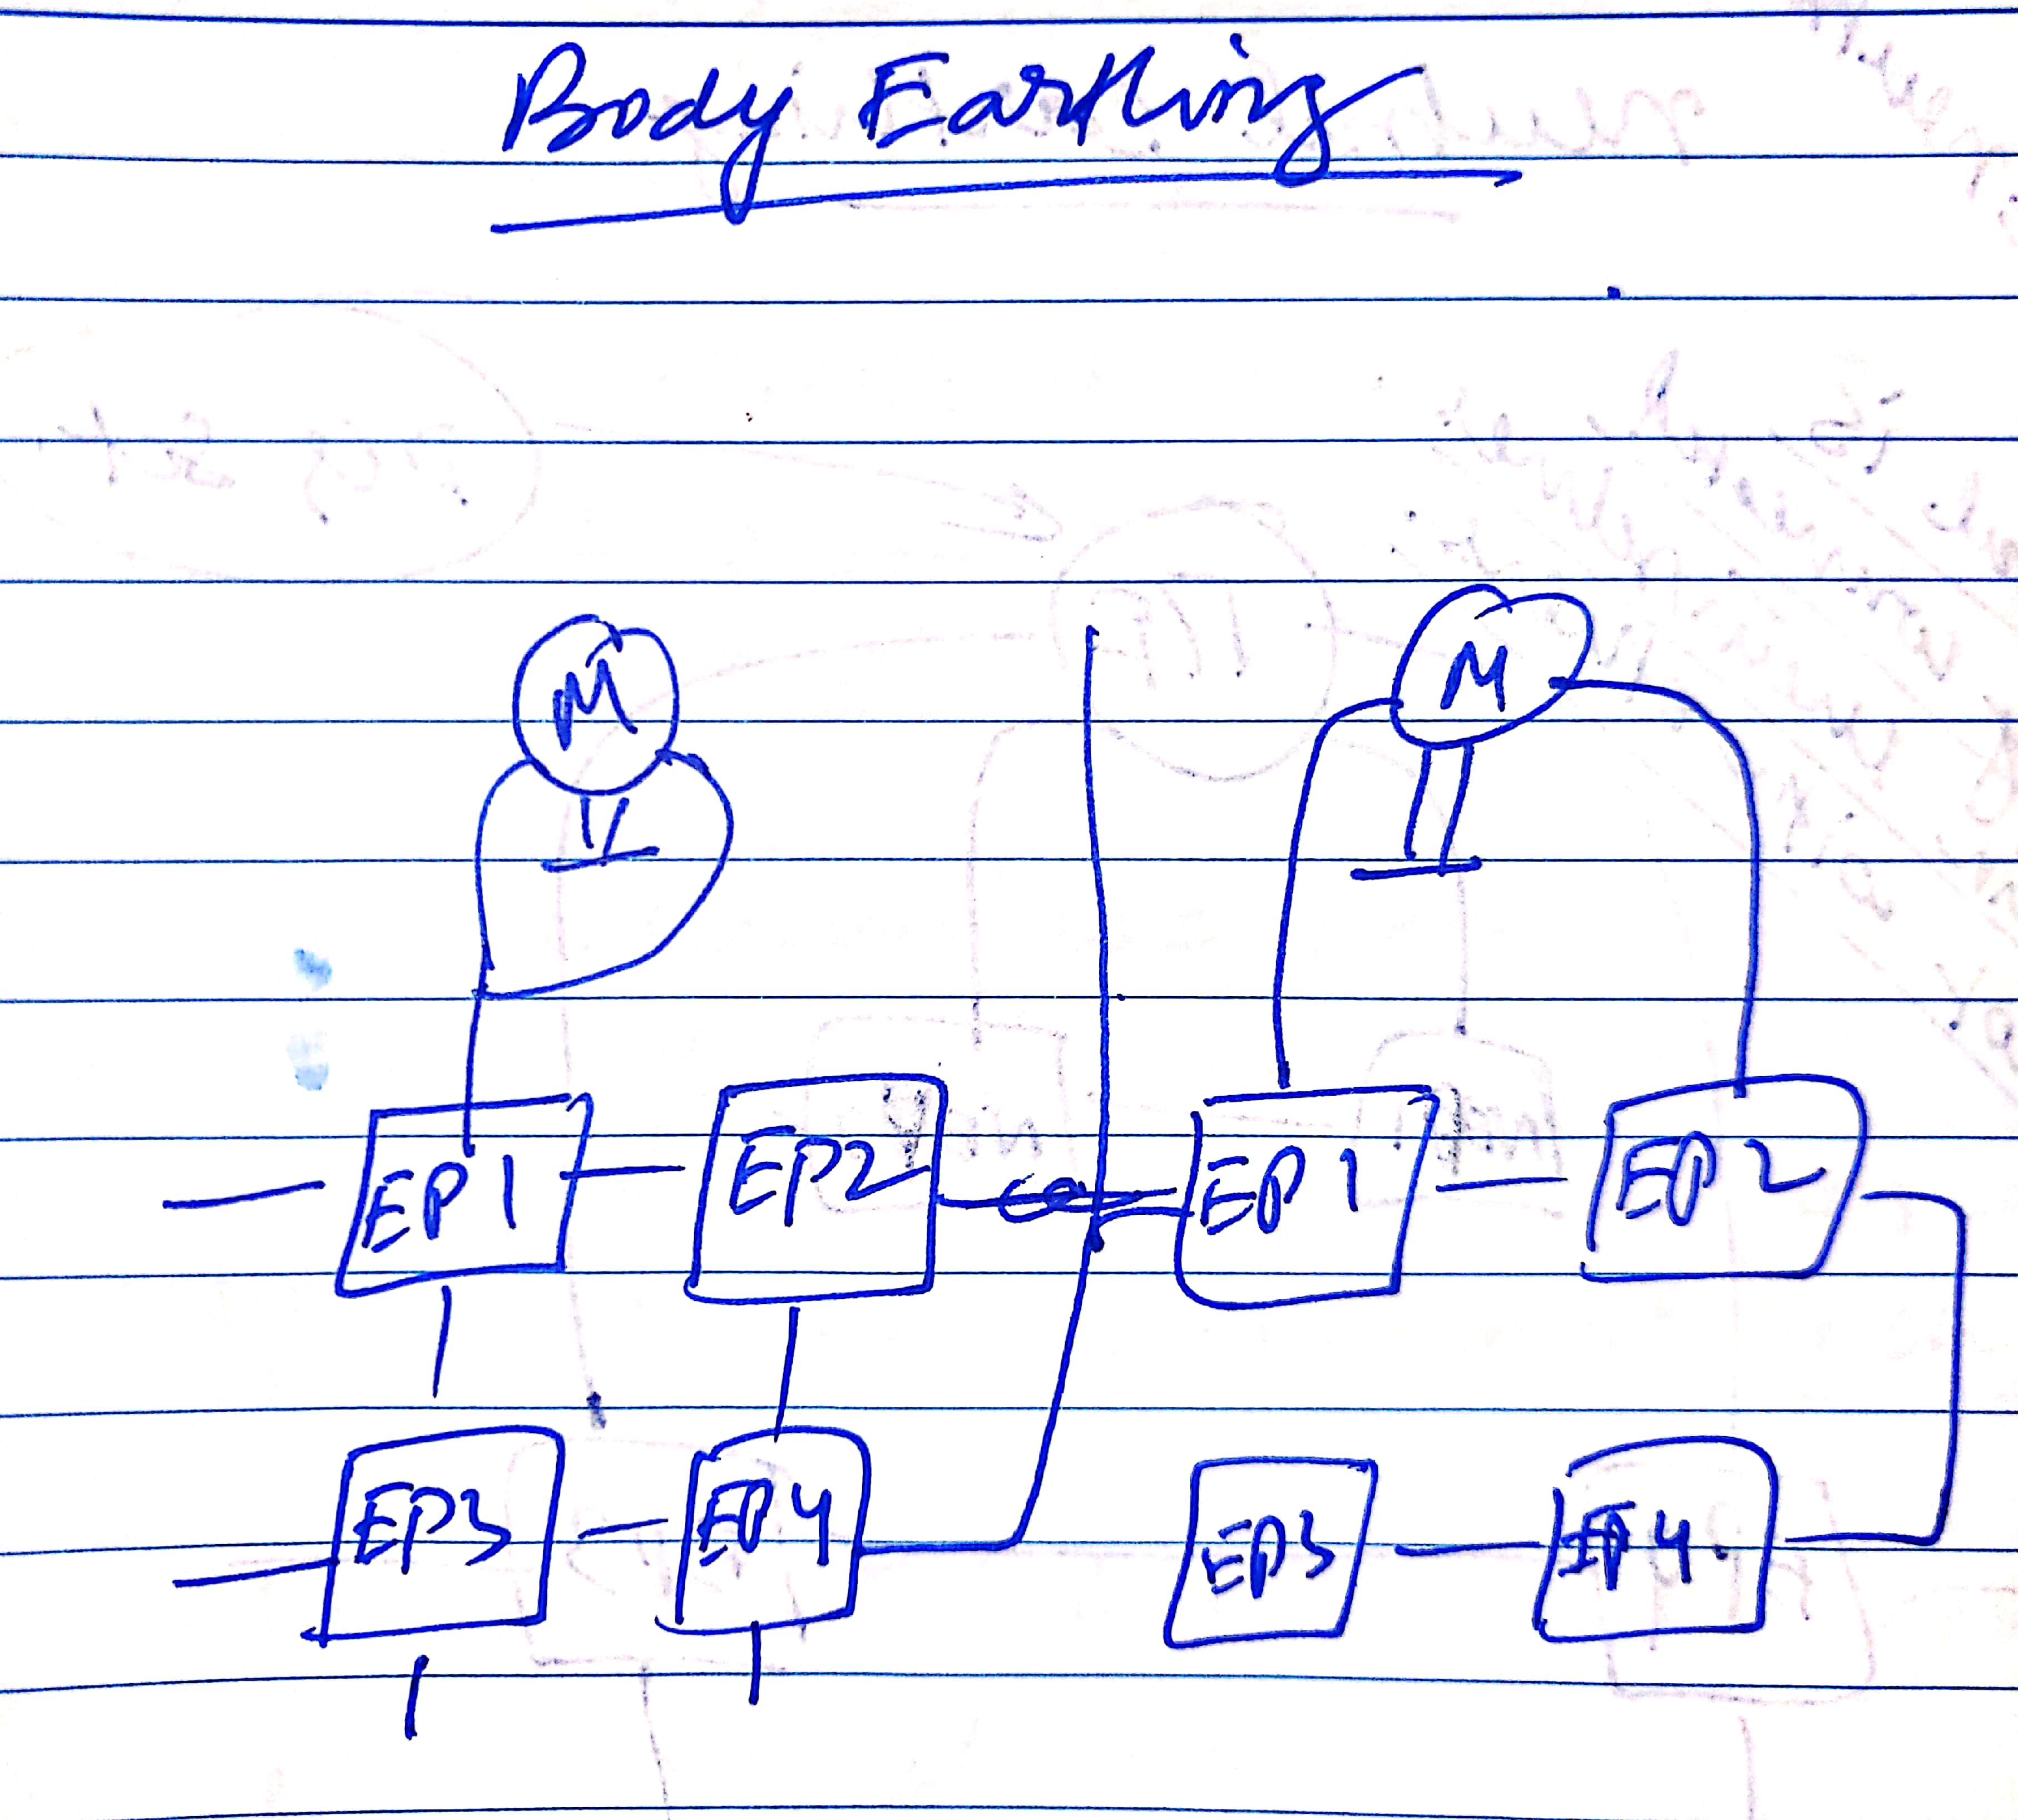
\includegraphics[height=10cm,width=0.33\linewidth]{body_earthing}\label{body_earthing}}
		\caption{Different types of earthing schemes}
		\label{bp_earthing}
	\end{figure}
	\begin{figure}[h]
		\centering
		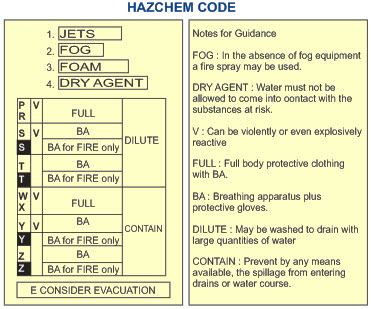
\includegraphics[width=0.5\linewidth]{hazchem}
		\caption{Hazchem decoded (BA=Breathing Apparatus)}
		\label{hazchem}
	\end{figure}
\chapter{Bareja Terminal}
	\section{Important Terms and Abbreviations}
	\begin{itemize}
		\item ROSOV= Remotely Operated Shut Off Valve
		\item DBBV= Double Block and Bleed Valve
		\item COCO= Company Owned and Company Operated
		\item PD Meter= Positive Displacement Meter
		\item DCV= Digital Control Valve
		\item BCU= Batch Control Unit
		\item MS= Motor Spirit (Petrol)
		\item HSD= High Speed Diesel 
		\item SKO= Superior Kerosene Oil
		\item ATF= Aviation Turbine Fuel
		\item MDG= Marketing Discipline Guidelines
		\item TLF= Tank Lorry Filling
		\item DCP= Dry Chemical Powder
		\item PPE= Personal Protection Equipment
	\end{itemize}
	\section{Operations}
	Operations at Bareja Terminal consists of the following things:-
	\begin{itemize}
		\item Receipt
		\item Storage
		\item Dispatch
		\item Quality
	\end{itemize}
	Each of these are described in further detail below.
	\subsection{Receipt}
	Bareja terminal receives product via 2 pipelines:-
	\begin{itemize}
		\item KSPL (Koyali- Sanganer Pipe Line) = Multiproduct pipeline tapped at Ahmedabad
		\item KAPL (Koyali- Ahmedabad Pipe Line) = Dedicated ATF pipeline which supplies the whole of Gujarat and parts of Rajasthan.
	\end{itemize}
	Then interface cutting (See Fig \ref{interface_cutting})is done by the pipelines division at the exchange pit and supplied to the terminal via pipelines. 
	\subsection{Storage}
	\begin{itemize}
		\item Tank farm at bareja terminal can be represented by Fig \ref{bareja_tank_farm}.
		\item The storage capacities of the aforementioned tanks can be realized by Table \ref{bareja_tank_cap}.
		\item Tanks are classified in 3 ways - 
		\begin{itemize}
			\item Underground and Aboveground tanks
			\item Floating roof tanks and cone roof tanks
			\item Horizontal and Vertical tanks
		\end{itemize}
		\item Floating roof tanks are used to store class A products such as MS, which are very volatile thereby prone to vapor loss. The floating roof of the tank floats just over the product thereby not giving any space for vapor to form.
		\item A floating roof tank has the following attachments to its roof with their specific purpose -
		\begin{itemize}
			\item Articulated Vent - to remove water stored on roof by rain or foam pouring drills etc.
			\item Primary seal - Metal (aluminum) clamps sealing the product in.
			\item Secondary seal - Secondary line of defense from product leakage and provides weather protection to the primary seal.
			\item Stands - So the floating roof doesn't touch the bottom of the tank when tank is emptied for cleaning or maintenance purposes (6ft length).
			\item Auto-bleeder valve - Leg length a bit longer than the stand and open cap on other side. This opens the valve when the floating roof lowers beyond a point thereby stopping vacuum locking.  
			\item For safety there are foam pourers and foam dams to direct foam towards the secondary seal which is most prone to product leakage and fire.
			\item There are automatically triggered (by the rate of increase of temperature) foam pourers which pour foam directly over the primary seal in case of an emergency.
		\end{itemize}
		\item The bottom of any tank has a central sump to collect any water that has infiltrated the system and a water draw off line to drain that water.
		\item The sand pad that forms the base of the tank should - have no cracks, have no vegetation since roots crack the base even further.
		\item A tank can be either of the 3 modes - Receipt, Dispatch and Dormant. (See Fig \ref{tank_modes})
		\item There are alarms for overfilling and underfilling of tanks, the details about which can be easily understood from Fig \ref{tank_alarms}.
		\item There are various valves attached to the inlet and the outlet of the tanks which can be seen in Fig \ref{tank_valves}. It is important to note here that the ROSOV can only be shutoff remotely but has to be turned on manually whereas the DBBV can be shutoff and turned on remotely and in case of loss of power, the ROSOV closes automatically. This is done, so that when someone manually opens the ROSOV, then that person can check the surroundings for any hazards before doing so.
	\end{itemize}
	\subsection{Dispatch}
	\begin{itemize}
		\item There are 2 types of customers - Retail Outlets, Bulk Consumers
		\item It is to be noted that product given to COCO ROs and AFS are treated as stock transfer rather than sale.
		\item Dispatch is done via tank trucks which can be - dealer owned, transporter owned and consortium owned.
		\item The demand sensing or indenting is done via sms or web indenting.
		\item ATF has dedicated tankers which is coated internally with epicoating to prevent chemical reaction with the tanker metal thereby contaminating it.
		\item The following is the priority list of the customers while dipatching loads to it - 
		\begin{enumerate}
			\item Consumer sales
			\item Priority dealers 
			\item COCO
			\item Non Priority dealers
		\end{enumerate}
		\item The complete flow of the TT coming in empty and leaving the automated terminal can be seen in Fig \ref{distribution_flow}.
		\item The filling of the TT can be further maginified to a process flow as seen in Fig \ref{filling_flow}.
		\item The instruments used to automatically fill the TTs along with their order of operation is shown in Fig \ref{tlf_flow}. The PD meter (sensor) supplies information to the BCU which then sends the open or close signal to the DCV (actuator). The DCV can either be open or close, anything in between is achieved by repeatedly turning the valve ON and OFF.
	\end{itemize}
	\subsection{Quality}
	The various stages at which quality checks are done can be seen in Fig \ref{bareja_quality_flow}.\par
	Batch formation test for MS,HSD,SKO :-
	\begin{itemize}
		\item Settling time of one hour
		\item Sample from Top, Bottom and Middle (TMB sampling)
		\item 9 different tests are performed
		\item Density, Distillation, Sulphur, Copper, ROE, Appearance, Color, RON
		\item Tests are carried Monthly, weekly and MDG
		\item Test reports are issued to Control Room
	\end{itemize}
	Batch formation test for ATF :- (Quality control is significantly more important in this case because of the huge risk of human lives)
	\begin{itemize}
		\item Settling time of two hours
		\item Sample from Upper, Lower and Middle
		\item 21 different tests are performed
		\item Tests are carried Monthly, weekly and MDG
		\item Test reports are issued to Control Room
		\item Every TT carries the test report
	\end{itemize}
	Checks done during TLF:-
	\begin{itemize}
		\item Density Checks (done by online density meter and by the TT crew in presence of officer)
		\item Dip Check (done by the TT crew for their own satisfaction)
		\item Water Check (only for ATF)
		\item Sediment Check (only for ATF)
	\end{itemize}
	Important quality points for different products :-
	\begin{itemize}
		\item MS,HSD : Density MS(720-775 kg/m3) HSD(815-845 kg/m3)
		\item SKO : Flashpoint (\ang{35}C)
		\item ATF : Water and sediment present only in tolerable limits
	\end{itemize}
	\section{Safety and Maintenance}
	\subsection{Cone Roof Tanks}
	\begin{itemize}
		\item Annuluar plate extension
		\item Air vent
		\item Water marks on roof 
		\item Earthing strip
		\item Sprinkler Systems
		\item Stair case and handrail
		\item Water Drains
		\item Sand pad foundation
		\item Tank cleaning
	\end{itemize}
	\subsection{Floating Roof Tanks}
	\begin{itemize}
		\item Pontoons
		\item Articulated drains
		\item PV valves
		\item Auto Bleeder vents
		\item Sprinkler system
		\item Primary and secondary seal
		\item Foam Dam
		\item Sand Pad Foundation
		\item Tank cleaning
	\end{itemize}
	\subsection{Pipeline Maintenance}
	\begin{itemize}
		\item There are 2 types of pipelines - Hydrant and Product lines
		\item Solid rod between pipe and foundation
		\item Guiding rods
		\item Wrapping coating in underground pipeline
		\item Inspection of pipeline foundation
		\item No Vegetation
		\item Pressure testing
		\item Clamps for leakage
		\item Cathodic Protection
		\item Route Lines
	\end{itemize}
	\subsection{Pumps Maintenance}
	\begin{itemize}
		\item Strainer Cleaning
		\item Vibration Check
		\item Temperature Checks
		\item Rubber mat
		\item Flame Protection
		\item Coupling guard
		\item Pump house manifold 
		\item Body Earthing
	\end{itemize}
	\subsection{Electrical Maintenance}
	\begin{itemize}
		\item Electrical Audit by CEA every 3 years
		\item Periodic change of transformer oil
		\item Periodic replacement of silica gel in transformers
	\end{itemize}
	\subsection{Safety Equipments}
	\begin{itemize}
		\item DCP Fire Extinguishers
		\item Medium Expansion Foam Generator (MEFG)
		\item High Velocity Long Range Monitor (HVLRM)
		\item Hydrocarbon Detectors
		\item Dyke valve indicator
		\item Level Alarms (HHH, HH, H, L, LL, LLL)
	\end{itemize}
	\subsection{Safety of TT}
	\begin{itemize}
		\item Hazardous Chemical handling certification
		\item Green Card
		\item Battery cut-off
		\item Master valve
		\item Emergency valve
		\item Safety lock
		\item Spark Arrestors
		\item Space between tanker and driver cabin
		\item Tank size less than drivers cabin
		\item Lead fire safety link
		\item Earthing
		\item Air vent
	\end{itemize}
	\subsection{Additional Safety Measures}
	\begin{itemize}
		\item Water Sprinkler System
		\item Emergency Alarms
		\item Fire Water Pump House
		\item Flame Proof Equipments
		\item Earthing
		\item Frisking
		\item Sand Buckets
		\item Follow SOP
		\item PPEs
	\end{itemize}
	
	\clearpage
	\pagebreak
	\section{Tables}
	\begin{table}[h]
		\centering
		\begin{tabular}{@{}llll@{}}
			\toprule
			\textbf{Storage Tank} & \textbf{Quantity} & \textbf{Level Filled (kL)} & \textbf{Tank Diameter (m)} \\ \midrule
			MS                    & 3                 & 8300                       & 24                         \\
			HSD                   & 4                 & 11000                      & 32                         \\
			ATF                   & 2                 & 6300                       & 28                         \\
			SKO                   & 2                 & 3300                       & 18                         \\
			Ethanol               & 2                 & 70                         &                            \\
			Water                 & 3                 & 2600/5200                  &                            \\ \bottomrule
		\end{tabular}
	\caption{Tank Capacities \& Storing Limit}
	\label{bareja_tank_cap}
	\end{table}
	\clearpage
	\pagebreak
	\section{Figures}
	\begin{figure}[h]
		\centering
		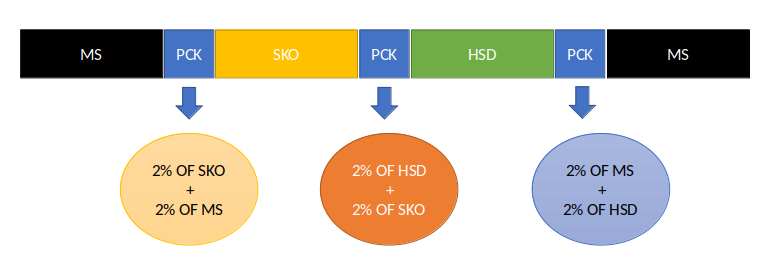
\includegraphics[width=\linewidth]{interface_cutting}
		\caption{Interface cutting norms}
		\label{interface_cutting}
	\end{figure}
	\begin{figure}[h]
		\centering
		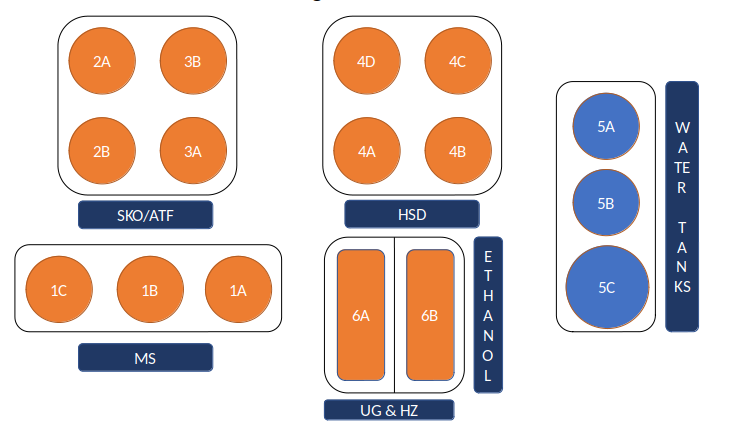
\includegraphics[width=\linewidth]{bareja_tank_farm}
		\caption{Pictorial representation of the storage tanks present at the Bareja terminal}
		\label{bareja_tank_farm}
	\end{figure}
	\begin{figure}[h]
		\centering
		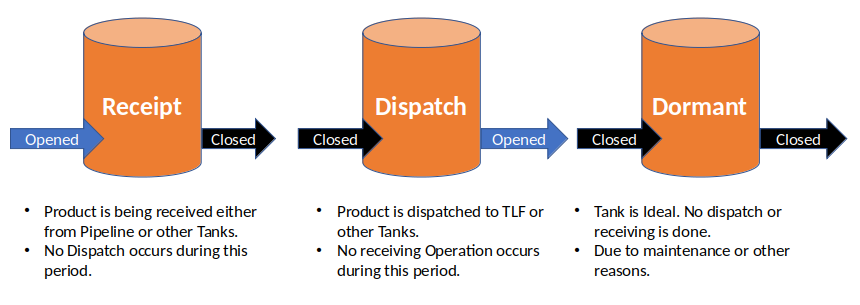
\includegraphics[width=\linewidth]{tank_modes}
		\caption{Modes of operation of tanks}
		\label{tank_modes}
	\end{figure}
	\begin{figure}[h]
		\centering
		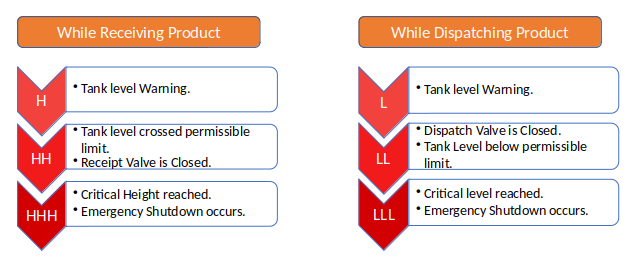
\includegraphics[width=\linewidth]{tank_alarms}
		\caption{Alarms to prevent over filling or over emptying a tank}
		\label{tank_alarms}
	\end{figure}
	\begin{figure}[h]
		\centering
		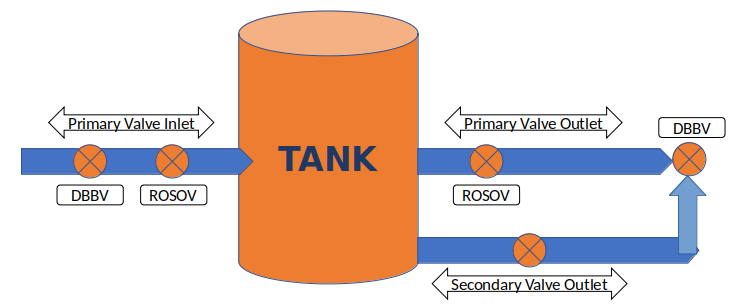
\includegraphics[width=\linewidth,height=5cm]{tank_valves}
		\caption{Valves attached to a tank}
		\label{tank_valves}
	\end{figure}
	\begin{figure}[h]
		\centering
		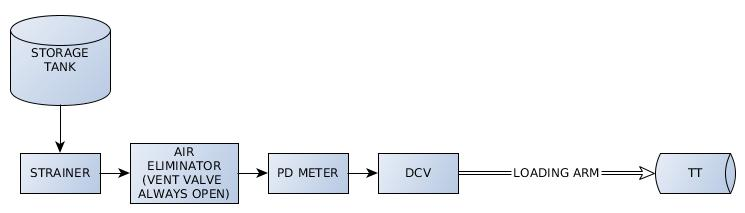
\includegraphics[width=\linewidth]{tlf_flow}
		\caption{Equipments and process flow enabling the completely automatic filling of TTs}
		\label{tlf_flow}
	\end{figure}
	\begin{figure}[h]
		\centering
		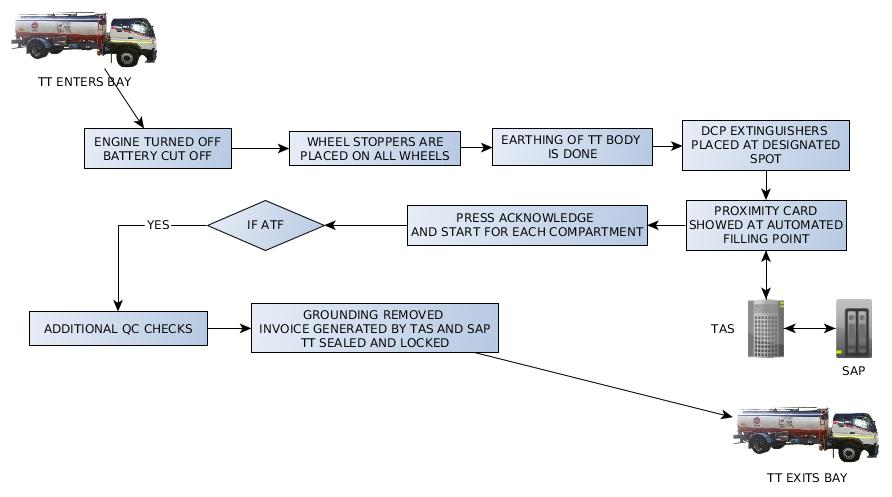
\includegraphics[width=\linewidth]{filling_flow}
		\caption{The TLF process flow (magnified to the filling part)}
		\label{filling_flow}
	\end{figure}
	\pagebreak
	\begin{landscape}
		\begin{figure}[h]
			\centering
			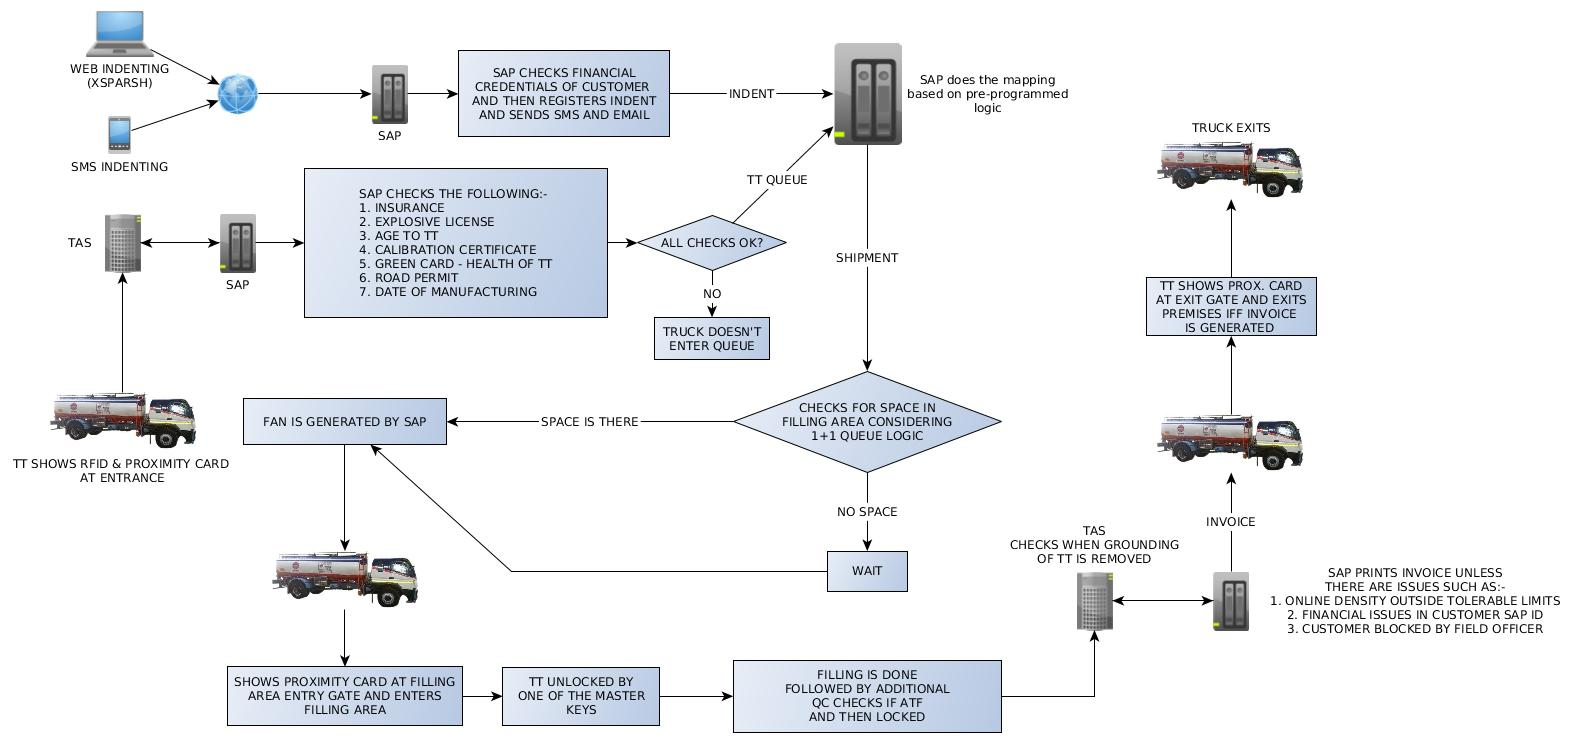
\includegraphics[width=\linewidth]{distribution_flow}
			\caption{The complete TLF process flow}
			\label{distribution_flow}
		\end{figure}
	\end{landscape}
	\pagebreak
	\begin{figure}[h]
		\centering
		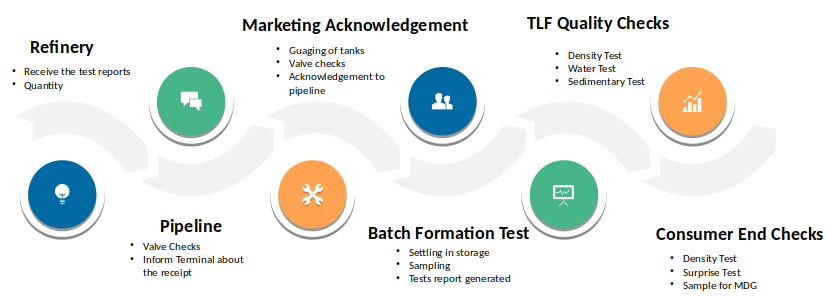
\includegraphics[width=\linewidth]{bareja_quality_flow}
		\caption{Quality flow at Bareja terminal}
		\label{bareja_quality_flow}
	\end{figure}
		\begin{figure}[h]
		\centering
		\subfloat[][Fire Triangle]{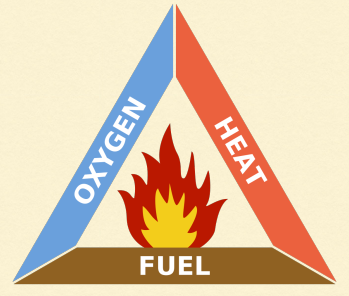
\includegraphics[height=5cm,width=5cm]{fire_triangle}\label{fire_triangle}}
		\subfloat[][Hierarchy of controls]{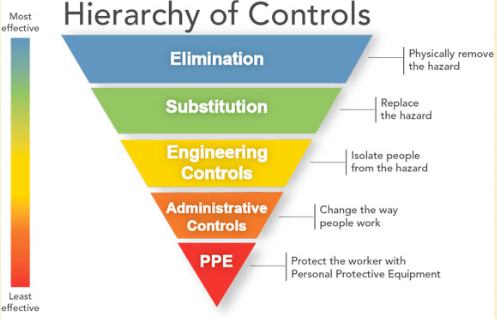
\includegraphics[height=5cm,width=5cm]{hierarchy_of_controls}\label{hierarchy_of_controls}}
		\caption{Major safety concepts}
		\label{major_safety_concepts}
		\end{figure}
	\chapter{LPG Distributorship}
	\section{Important Terms and Abbreviations}
	\begin{itemize}
		\item POI= Proof of Identity
		\item POA= Proof of Address
		\item RSP= Retail Selling Price
		\item PDC= Pre Delivery Check
	\end{itemize}
	\section{Salient Points about the LPG Distribution Operation}
	\begin{itemize}
		\item Distributors are expected to be ``sellers"
		\item Distributor has a office (showroom) and a godown
		\item Flame lighters are much better than spark lighters since they provide a continuous flame and donot allow for any gas leakage before ignition. However they have couple of disadvantages as are listed below:-
		\begin{itemize}
			\item They have to be refueled 
			\item Fuel level is not visible so it can stop working anytime
			\item Not an easily marketable product since it has cheap replacements such as a matchstick or a simple lighter
			\item Can be easily replaced by filament based electrical lighter which could be charged by the customer as his/her ease.
			\item Flame lighters are not very durable due to their complicated mechanism of working.
		\end{itemize}
		\item The following documents are required by any distributor in order to run their operation -
		\begin{itemize}
			\item Fire license
			\item Trade license
			\item Retail selling license (for certain states) 
			\item Shop and establishment license
		\end{itemize}
		\item The following documents are required from the customer in order to get a new connection :-
		\begin{itemize}
			\item POI
			\item POA
			\item KYC Form
			\item Aadhar Card (if subsidy is required)
		\end{itemize}
		\item If there are 3 stay plates, its a PSU cylinder and if there are 4 stay plates, its a private OMC cylinder
		\item Cylinder classification based on Shroud colour - BPC is Yellow, HPC is Blue and IOCL has no seperate colour 
		\item Documents generated at a distributorship:-
		\begin{itemize}
			\item SV= Subscription Voucher - acknowledgment for deposit of voucher
			\item TV= Termination Voucher - deposit comes back
			\item TTV= Transfer Termination Voucher - deposit doesn't come back
			\item TSV= Transfer Subscription Voucher - deposit is not required
		\end{itemize}
		\item A distributor should have 1 platform weighing scale at godown and all the delivery boys should have one portable weighing scale.
		\item The capacity of a distrubutor's godown is the amount of gas he is allowed to keep. For eg. 8000 kg means 8000kg/14.2kg= 564 filled cylinders to be kept.
		\item RSP is the only price that can be charged for a cylinder. Only, the district distributor can give permit to collect charges over and above RSP.
		\item Grievance Redressal phone number for all three OMCs : 1800 2333 555 (not for leakage)
		\item According to the Unified Selection Guidelines, there are 4 types of LPG distributorships - Sahari Vikrats, Rurban Vikrats, Gramin Vikrats and Durgam Shetriya Vikrats
		\item Percentage of location allocation between the three OMCs - 50\% for IOCL , 25\% for BPCL, 25\% for HPCL.
		\item The customer ID remains same when a customer shifts from one OMC to another OMC under the portability scheme, only the customer number changes.
		\item During delivery of the cylinders to the warehouse, 10\% of the cylinders should be checked for underwieght (max -100 g) and overweight (max +200 g).
		\item During delivery of the cylinders to the customer's premises, all the cylinders should go through PDC which includes- weight check, o ring leak check, valve leak check.
		\item The distributorship software is being shifted from Insoft to SDMS on a selective rollout basis.
		\item The number to call to book a cylinder - (96)24365365 where the 96 part changes according to the state, but the rest remains same - 24 hours a day for 365 days therefore 24 365 365.
		\item The cash and carry rebate is Rs. 24.05 currently.
		\item The pricing details of the various aspects of domestic LPG distribution is given in Table \ref{lpg_price}. In Ujjawala scheme, the govt pays for the deposit - cylinder and pressure regulator which is not recovered. However, the first free Gas Refill and Stove cost is paid by the OMC and recovered by absorbing subsidies. The hose and DGCC is paid for by OMC and not recovered. So initially, the ujjawala customer only has to pay the franking cost and later couple of sibsidies are absorbed.
	\end{itemize}
	\section{Tables}
	\begin{table}[H]
		\centering
		\begin{tabular}{@{}lll@{}}
			\toprule
			\textbf{S. No.} & \textbf{Item}                                                                                 & \textbf{\begin{tabular}[c]{@{}l@{}}Price in Rs. \\ (inclusive of GST)\end{tabular}}                        \\ \midrule
			1               & Cylinder Deposit                                                                              & 1450                                                                                                       \\
			2               & Pressure Regulator Deposit                                                                    & 150                                                                                                        \\
			3               & DGCC Book                                                                                     & 59                                                                                                         \\
			4               & Installation and Administration                                                               & 118                                                                                                        \\
			5               & Admin Charges                                                                                 & 88.5                                                                                                       \\
			6               & Suraksha Hose 1.5m (normal)                                                                   & 190                                                                                                        \\
			7               & Suraksha Hose 1.2m (Ujjawala)                                                                 & 170                                                                                                        \\
			8               & \begin{tabular}[c]{@{}l@{}}Stove inspection charges if stove is \\ \\ not bought\end{tabular} & \begin{tabular}[c]{@{}l@{}}1 burner = 100 + GST \\ \\ then for each burner \\ \\ 50 is added.\end{tabular} \\
			9               & Franking Cost on SV                                                                           & 300                                                                                                        \\
			10              & Ujjawala Stove (2 burner)                                                                     & 990                                                                                                        \\ \bottomrule
		\end{tabular}
		\caption{Various pricing elements in domestic LPG distribution}
		\label{lpg_price}
	\end{table}
	\chapter{Gujarat Refinery}
	\section{Important Terms and Abbreviations}
	\begin{itemize}
		\item AU= Atmospheric Unit
		\item LGO= Light Gas Oil
		\item HGO= Heavy Has Oil
		\item DHDT= Diesel HyDro Treater
		\item SRU= Sulphur Recovery Unit
	\end{itemize}
	\section{Salient points about Gujarat Refinery}
	\begin{itemize}
		\item Total capacity = 13.7 MMTPA (the amount of crude it can process)
		\item All India IOCL capacity = 80.70 MMTPA but will be increased 100+ MMTPA (in 5 years)
		\item Land size = 1000 acre
		\item 80\% crude is imported by IB Department
		\item Crude comes only in pipeline due to financial reasons
		\item Earlier kerosene was the main product but with the introduction of electrical lighting and internal combustion engines, the main product shifted to MS,HSD. Then began the slow declination of sulphur. All this means the refinery operation is highly dynamic
		\item Feedback from marketing department helps in refinery product optimization.
		\item The three things required for successful refinery operation - Equipment, Energy, Employee
		\item The refinery has a captive power plant of 120 MW
		\item Maximum capacity of tankage present in refinery is 5000 kL
		\item A desalter is a device which removes salt by density difference via electrostatic precipitator.
	\end{itemize}
	The refinery process flow is summarized in Fig \ref{refinery_flow}.
	\section{Sulphur removal from fuel}
	To remove sulphur from fuel, we need to react the fuel with hydrogen. This hydrogen we get from the chemical reaction - \par
	\ch{CH4 + H2O ->[catalyst] CO + 3 H2 (gas)}\par
	This reaction occurs in the reformer unit.
	The \ch{CH4} here cannot have any higher hydrocarbon or it would poison the catalyst. Therefore, to remove any higher hydrocarbon we need a pre-reformer unit.\par
	The pre-reformer unit removes all higher hydrocarbons from the \ch{CH4} feed, however, if there is sulphur in the feed, it will poison the catalyst. Therefore, to remove sulphur from the feed we need a desulphurisation which required much less hydrogen.
	
	The process flow of the sulphur removal process can be seen in Fig \ref{sulphur_removal_flow}.
	\clearpage
	\pagebreak
	\section{Figures}
	\begin{figure}[h]
		\centering
		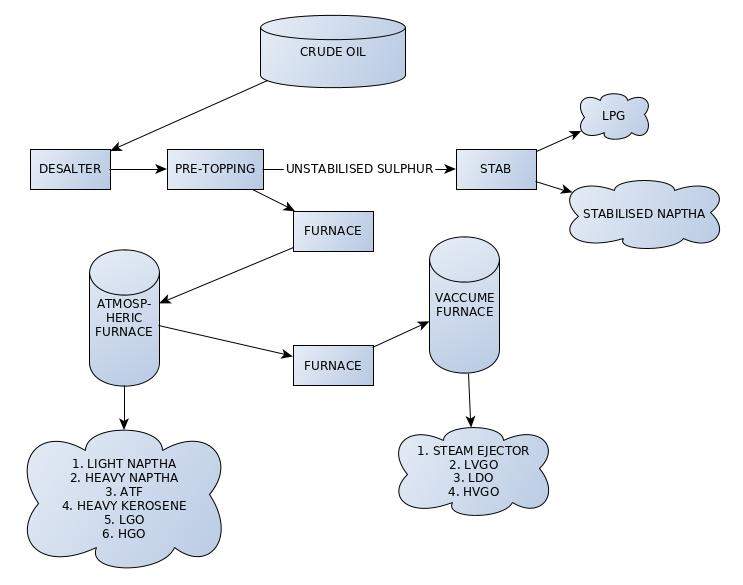
\includegraphics[width=\linewidth,height=13cm]{refinery_flow}
		\caption{Brief process flow of refinery operations}
		\label{refinery_flow}
	\end{figure}
	\begin{figure}[h]
		\centering
		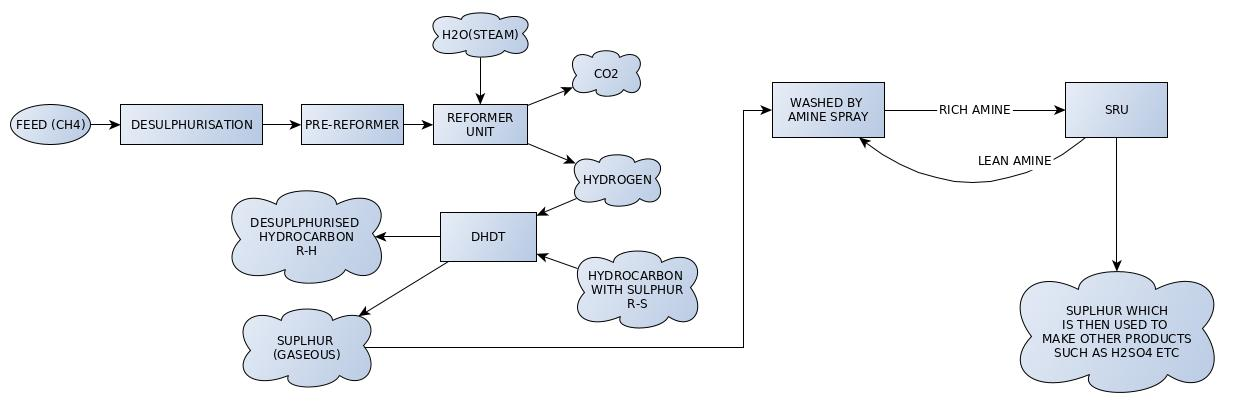
\includegraphics[width=\linewidth]{sulphur_removal_flow}
		\caption{Process flow of the fuel desulphurisation operation in refinery}
		\label{sulphur_removal_flow}
	\end{figure}
	\chapter{FAQs}
	\begin{enumerate}
		\item What is the standard pressure in a LPG T/T?
		\item What is the minimum pressure in a LPG cylinder?
		\item What factors go into the calculation of production requirement of a bottling plant?
		\item Why are LOT cylinders required?
		\item What is the additive added to LPG in Nanocut cylinder and what parameter of the LPG does it change?
		\item What is MSDS of a product?
		\item What principle is used in LPG TT decantation ?
		\item Being an odourless product, why does LPG have a particular odour ?
		\item What is UEL and LEL for LPG?
		\item What is BLEVE ?
		\item What is UVCE? - Unconfined Vapour Cloud Explosion
		\item Why is EFCV placed inside and outside the body of the TT now-a-days?
		\item What is the function of SC valve?
		\item What are three methods of fire control? 
		\item What is the OISD standard code for LPG? - OISD 144
		\item What is the emergency LPG leakage contact number?
		\item What is STP?
		\item What is the Door Drishti Programme? - automated software which gives OLD (o ring detector) and VLD (valve ring detector) details
		\item What is the purpose of unlicensed and licensed areas in plants/terminals?
		\item What are the documents required by the tank trucks?
		\item What are the documents required by the LPG cylinder distribution trucks?
		\item Which kind of flooring is required in shed and godown?
		\item What pressure is maintained in the hydrant lines?
		\item Why don’t bullets face any other facilities?
		\item What is the function of Roto-gauge?
		\item What is the purpose of sprinkler systems on LPG storage tanks?
		\item What percentage of space should be present in LPG storage vessel/TT?
		\item Why are cylinder deshaped before scrapping?
		\item Which body formulates the norms for STP?
		\item Why is soap solution used for lubrication of chains in conveyer belts in LPG BP?
		\item What is GMS?
		\item What is SCABA? - Self Contained Air Breathing Apparatus
		\item What is LOTO and why is it required?
		\item What is the hazchem code for LPG? - 2WE
		\item What is breakaway coupling?
		\item What is the purpose of jockey pumps?
		\item What is the requirement of LL and LLL alarm?
		\item What are basic operation of Terminal?
		\item What is bridging?
		\item Why is floating roof tank used in MS?
		\item What is stock loss and stock gain? - volume change of LPG due to temp change
		\item What is ROSOV and DBBV?
		\item What are the 4 modes of operation of a storage tank? - receipt, dispatch, dormant, under maintainance 
		\item What is the purpose of secondary outlet in storage tanks of MS/HSD?
		\item What is single contingency and double contingency?
		\item Why to blend ethanol?
		\item What are the sources of ethanol?
		\item What additive is added to ethanol to make is toxic and thereby rendering it unfit for consumption? - Crotonaldehyde
		\item What is the purpose of secondary seal? - 2nd line of defence and weatherproofing primary seal
		\item What are pontoons and why are they required?
		\item What is the difference in operating paramters of ACB and VCB?
		\item At what oil and winding temperature does the overheat sensor set off an alarm and trip?
		\item What is the ideal colour of silica gel used in transformers? - blue colour
		\item What is principle of automatic trigerring of foam pouring system onto primary seal? 
		\item Which thermometer is required for density testing ? - IP64C
		\item What are the ways to place indent?
		\item What is the difference between TMB and UML sampling?
		\item What is the difference between PCK and SKO? - PCK has less sulphur content and can be mixed with MS, HSD or SKO
		\item What is the most durable identification of Indane cylinders? - 6 horizontal oval holes in the footring
		\item What are the fire protection systems at place in godowns?
		\item What are the prequalifications required for a party to participate in public tender?
		\item What is the purpose of sand bitumen mixture between concrete foundation and annular plate extension of storage tanks?
		\item What is the function of saddle plates in pipelines?
		\item What is the testing pressure of pipelines? - 1.5 times for water , 1.1 times for product ; the operating pressure
		\item Where is cathodic protection used?
		\item What is function of quartzoid bulb?
		\item What are the types of pricing for aviation fuels?
		\item What are the two mthods of filling avitation fuel into the aircraft?
		\item Who is the main authority of all aviation related matters in India?
		\item What is floating suction in ATF and why is it used?
		\item What is function of air vent and free vent ?
		\item What is function of tail-tale hole?
		\item Which test is done before decantation of ATF TT?
		\item What is Deadman switch and why is it required?
		\item What are the personnel present during refuelling? - driver, operator, officer, aircraft maintainence officer
		\item What are the two critical checks in ATF?
		\item Why does all ATF storage vessels require epicoating?
		\item What is the colour change of aquades capsule? - colourless to pink in presence of water
		\item What is PTO gear?
		\item Why is brake interlock system required in aviation refuellers?
		\item How much sediments are allowed in ATF as per IOCL norms? - 0.2 mg/l (1 mg/l as per IATA norms)
		\item How much water is allowed in ATF as per IOCL norms? - 15 ppm (30 ppm as per IATA norms)
		\item What is allowable density variation in ATF?  -  +/- 2.5 kg/m3
		\item What is hazchem code for ATF? - 3YE
		\item Why are spark lighters being replaced by flame lighters?
		\item What are the statutory licenses required for LPG distributorship? - fire license, trade license, retail selling license (for certain states) , shop and establishment license
		\item What are the documents to be collected from new customers? - POI, POA, KYC, Aadhar(for subsidy)
		\item What are the classifications of LPG distributors as per USG?
		\item Can distributors take loads on credit and how ?
		\item What is the number for IVR booking? - (96)24365365  96 is dependent on state
		\item What are the PDCs? - o ring check, valve leak check, weight check
		\item What is the technical name of the bluebook which a LPG customer has? - DGCC book (Domestic Gas Consumer Card)
		\item What are NDNE retailer? - standalone commercial retailers
		\item What are godown stacking guidelines? - filled 25 X 4 X 2 , empty 25 X 4 X 2 or 3
		\item Where is LAB(Linear Alkyle Benzene) used ? - detergents
		\item What is the mother unit of refineries? - AU
		\item What is the chemical used to convert gaseous H2S to liquid for physical seperation? - washed with amine to form rich amine
		\item How many hours of fire fighting capacity is required at any facility? - 4 hours
		\item What is the replacement of Insoft which is being rolled out to LPG distributors on a pilot basis?
		\item What is the ceiling limit of sale of a distributor?
		\item What is flash point, smoke point and fire point?
		\item uHow do we check RON and cetane number?
	\end{enumerate}
\end{document}